\documentclass[twoside]{book}

%%%%%%%%%%%%%%%%%%%%%%%%%%%%%%%%%%%%%%%%%
% The Legrand Orange Book
% Structural Definitions File
% Version 2.0 (9/2/15)
%
% Original author:
% Mathias Legrand (legrand.mathias@gmail.com) with modifications by:
% Vel (vel@latextemplates.com)
% 
% This file has been downloaded from:
% http://www.LaTeXTemplates.com
%
% License:
% CC BY-NC-SA 3.0 (http://creativecommons.org/licenses/by-nc-sa/3.0/)
%
%%%%%%%%%%%%%%%%%%%%%%%%%%%%%%%%%%%%%%%%%

%----------------------------------------------------------------------------------------
%	VARIOUS REQUIRED PACKAGES AND CONFIGURATIONS
%----------------------------------------------------------------------------------------

\usepackage[top=2.0cm,bottom=2.0cm,left=2.5cm,right=2cm,headsep=10pt,a4paper]{geometry} % Page margins

\usepackage{graphicx} % Required for including pictures
\graphicspath{{Pictures/}} % Specifies the directory where pictures are stored

\usepackage{lipsum} % Inserts dummy text

\usepackage{tikz} % Required for drawing custom shapes

\usepackage[english]{babel} % English language/hyphenation

\usepackage{enumitem} % Customize lists
\setlist{nolistsep} % Reduce spacing between bullet points and numbered lists

\usepackage{booktabs} % Required for nicer horizontal rules in tables

\usepackage{xcolor} % Required for specifying colors by name
% \definecolor{ocre}{RGB}{45,74,110} % Define the orange color used for highlighting throughout the book
\definecolor{ocre}{HTML}{3F729B}

%----------------------------------------------------------------------------------------
%	FONTS
%----------------------------------------------------------------------------------------

\usepackage{avant} % Use the Avantgarde font for headings
%\usepackage{times} % Use the Times font for headings
\usepackage{mathptmx} % Use the Adobe Times Roman as the default text font together with math symbols from the Sym­bol, Chancery and Com­puter Modern fonts

\usepackage{microtype} % Slightly tweak font spacing for aesthetics
\usepackage[utf8]{inputenc} % Required for including letters with accents
\usepackage[T1]{fontenc} % Use 8-bit encoding that has 256 glyphs

%----------------------------------------------------------------------------------------
%	BIBLIOGRAPHY AND INDEX
%----------------------------------------------------------------------------------------

\usepackage[style=alphabetic,citestyle=numeric,sorting=nyt,sortcites=true,autopunct=true,hyperref=true,abbreviate=false,backend=biber]{biblatex}
\addbibresource{bibliography.bib} % BibTeX bibliography file
\defbibheading{bibempty}{}

\usepackage{calc} % For simpler calculation - used for spacing the index letter headings correctly
\usepackage{makeidx} % Required to make an index
\makeindex % Tells LaTeX to create the files required for indexing

%----------------------------------------------------------------------------------------
%	MAIN TABLE OF CONTENTS
%----------------------------------------------------------------------------------------

\usepackage{titletoc} % Required for manipulating the table of contents

\contentsmargin{0cm} % Removes the default margin

% Part text styling
\titlecontents{part}[0cm]
{\addvspace{20pt}\centering\large\bfseries}
{}
{}
{}

% Chapter text styling
\titlecontents{chapter}[1.25cm] % Indentation
{\addvspace{12pt}\large\sffamily\bfseries} % Spacing and font options for chapters
{\color{ocre!60}\contentslabel[\Large\thecontentslabel]{1.25cm}\color{ocre}} % Chapter number
{\color{ocre}}  
{\color{ocre!60}\normalsize\;\titlerule*[.5pc]{.}\;\thecontentspage} % Page number

% Section text styling
\titlecontents{section}[1.25cm] % Indentation
{\addvspace{3pt}\sffamily\bfseries} % Spacing and font options for sections
{\contentslabel[\thecontentslabel]{1.25cm}} % Section number
{}
{\hfill\color{black}\thecontentspage} % Page number
[]

% Subsection text styling
\titlecontents{subsection}[1.25cm] % Indentation
{\addvspace{1pt}\sffamily\small} % Spacing and font options for subsections
{\contentslabel[\thecontentslabel]{1.25cm}} % Subsection number
{}
{\ \titlerule*[.5pc]{.}\;\thecontentspage} % Page number
[]

% List of figures
\titlecontents{figure}[0em]
{\addvspace{-5pt}\sffamily}
{\thecontentslabel\hspace*{1em}}
{}
{\ \titlerule*[.5pc]{.}\;\thecontentspage}
[]

% List of tables
\titlecontents{table}[0em]
{\addvspace{-5pt}\sffamily}
{\thecontentslabel\hspace*{1em}}
{}
{\ \titlerule*[.5pc]{.}\;\thecontentspage}
[]

%----------------------------------------------------------------------------------------
%	MINI TABLE OF CONTENTS IN PART HEADS
%----------------------------------------------------------------------------------------

% Chapter text styling
\titlecontents{lchapter}[0em] % Indenting
{\addvspace{15pt}\large\sffamily\bfseries} % Spacing and font options for chapters
{\color{ocre}\contentslabel[\Large\thecontentslabel]{1.25cm}\color{ocre}} % Chapter number
{}  
{\color{ocre}\normalsize\sffamily\bfseries\;\titlerule*[.5pc]{.}\;\thecontentspage} % Page number

% Section text styling
\titlecontents{lsection}[0em] % Indenting
{\sffamily\small} % Spacing and font options for sections
{\contentslabel[\thecontentslabel]{1.25cm}} % Section number
{}
{}

% Subsection text styling
\titlecontents{lsubsection}[.5em] % Indentation
{\normalfont\footnotesize\sffamily} % Font settings
{}
{}
{}

%----------------------------------------------------------------------------------------
%	PAGE HEADERS
%----------------------------------------------------------------------------------------

\usepackage{fancyhdr} % Required for header and footer configuration

\pagestyle{fancy}
\renewcommand{\chaptermark}[1]{\markboth{\sffamily\normalsize\bfseries\chaptername\ \thechapter.\ #1}{}} % Chapter text font settings
\renewcommand{\sectionmark}[1]{\markright{\sffamily\normalsize\thesection\hspace{5pt}#1}{}} % Section text font settings
\fancyhf{} \fancyhead[LE,RO]{\sffamily\normalsize\thepage} % Font setting for the page number in the header
\fancyhead[LO]{\rightmark} % Print the nearest section name on the left side of odd pages
\fancyhead[RE]{\leftmark} % Print the current chapter name on the right side of even pages
\renewcommand{\headrulewidth}{0.5pt} % Width of the rule under the header
\addtolength{\headheight}{2.5pt} % Increase the spacing around the header slightly
\renewcommand{\footrulewidth}{0pt} % Removes the rule in the footer
\fancypagestyle{plain}{\fancyhead{}\renewcommand{\headrulewidth}{0pt}} % Style for when a plain pagestyle is specified

% Removes the header from odd empty pages at the end of chapters
\makeatletter
\renewcommand{\cleardoublepage}{
\clearpage\ifodd\c@page\else
\hbox{}
\vspace*{\fill}
\thispagestyle{empty}
\newpage
\fi}

%----------------------------------------------------------------------------------------
%	THEOREM STYLES
%----------------------------------------------------------------------------------------

\usepackage{amsmath,amsfonts,amssymb,amsthm} % For math equations, theorems, symbols, etc

\newcommand{\intoo}[2]{\mathopen{]}#1\,;#2\mathclose{[}}
\newcommand{\ud}{\mathop{\mathrm{{}d}}\mathopen{}}
\newcommand{\intff}[2]{\mathopen{[}#1\,;#2\mathclose{]}}
\newtheorem{notation}{Notation}[chapter]

% Boxed/framed environments
\newtheoremstyle{ocrenumbox}% % Theorem style name
{0pt}% Space above
{0pt}% Space below
{\normalfont}% % Body font
{}% Indent amount
{\small\bf\sffamily\color{ocre}}% % Theorem head font
{\;}% Punctuation after theorem head
{0.25em}% Space after theorem head
{\small\sffamily\color{ocre}\thmname{#1}\nobreakspace\thmnumber{\@ifnotempty{#1}{}\@upn{#2}}% Theorem text (e.g. Theorem 2.1)
\thmnote{\nobreakspace\the\thm@notefont\sffamily\bfseries\color{black}---\nobreakspace#3.}} % Optional theorem note
\renewcommand{\qedsymbol}{$\blacksquare$}% Optional qed square

\newtheoremstyle{blacknumex}% Theorem style name
{5pt}% Space above
{5pt}% Space below
{\normalfont}% Body font
{} % Indent amount
{\small\bf\sffamily}% Theorem head font
{\;}% Punctuation after theorem head
{0.25em}% Space after theorem head
{\small\sffamily{\tiny\ensuremath{\blacksquare}}\nobreakspace\thmname{#1}\nobreakspace\thmnumber{\@ifnotempty{#1}{}\@upn{#2}}% Theorem text (e.g. Theorem 2.1)
\thmnote{\nobreakspace\the\thm@notefont\sffamily\bfseries---\nobreakspace#3.}}% Optional theorem note

\newtheoremstyle{blacknumbox} % Theorem style name
{0pt}% Space above
{0pt}% Space below
{\normalfont}% Body font
{}% Indent amount
{\small\bf\sffamily}% Theorem head font
{\;}% Punctuation after theorem head
{0.25em}% Space after theorem head
{\small\sffamily\thmname{#1}\nobreakspace\thmnumber{\@ifnotempty{#1}{}\@upn{#2}}% Theorem text (e.g. Theorem 2.1)
\thmnote{\nobreakspace\the\thm@notefont\sffamily\bfseries---\nobreakspace#3.}}% Optional theorem note

% Non-boxed/non-framed environments
\newtheoremstyle{ocrenum}% % Theorem style name
{5pt}% Space above
{5pt}% Space below
{\normalfont}% % Body font
{}% Indent amount
{\small\bf\sffamily\color{ocre}}% % Theorem head font
{\;}% Punctuation after theorem head
{0.25em}% Space after theorem head
{\small\sffamily\color{ocre}\thmname{#1}\nobreakspace\thmnumber{\@ifnotempty{#1}{}\@upn{#2}}% Theorem text (e.g. Theorem 2.1)
\thmnote{\nobreakspace\the\thm@notefont\sffamily\bfseries\color{black}---\nobreakspace#3.}} % Optional theorem note
\renewcommand{\qedsymbol}{$\blacksquare$}% Optional qed square
\makeatother

% Defines the theorem text style for each type of theorem to one of the three styles above
\newcounter{dummy} 
\numberwithin{dummy}{section}
\theoremstyle{ocrenumbox}
\newtheorem{theoremeT}[dummy]{Theorem}
\newtheorem{problem}{Problem}[chapter]
\newtheorem{exerciseT}{Exercise}[chapter]
\theoremstyle{blacknumex}
\newtheorem{exampleT}{Example}[chapter]
\theoremstyle{blacknumbox}
\newtheorem{vocabulary}{Vocabulary}[chapter]
\newtheorem{definitionT}{Definition}[section]
\newtheorem{corollaryT}[dummy]{Corollary}
\theoremstyle{ocrenum}
\newtheorem{proposition}[dummy]{Proposition}

%----------------------------------------------------------------------------------------
%	DEFINITION OF COLORED BOXES
%----------------------------------------------------------------------------------------

\RequirePackage[framemethod=default]{mdframed} % Required for creating the theorem, definition, exercise and corollary boxes

% Theorem box
\newmdenv[skipabove=7pt,
skipbelow=7pt,
backgroundcolor=black!5,
linecolor=ocre,
innerleftmargin=5pt,
innerrightmargin=5pt,
innertopmargin=5pt,
leftmargin=0cm,
rightmargin=0cm,
innerbottommargin=5pt]{tBox}

% Exercise box	  
\newmdenv[skipabove=7pt,
skipbelow=7pt,
rightline=false,
leftline=true,
topline=false,
bottomline=false,
backgroundcolor=ocre!10,
linecolor=ocre,
innerleftmargin=5pt,
innerrightmargin=5pt,
innertopmargin=5pt,
innerbottommargin=5pt,
leftmargin=0cm,
rightmargin=0cm,
linewidth=4pt]{eBox}	

% Definition box
\newmdenv[skipabove=7pt,
skipbelow=7pt,
rightline=false,
leftline=true,
topline=false,
bottomline=false,
linecolor=ocre,
innerleftmargin=5pt,
innerrightmargin=5pt,
innertopmargin=0pt,
leftmargin=0cm,
rightmargin=0cm,
linewidth=4pt,
innerbottommargin=0pt]{dBox}	

% Corollary box
\newmdenv[skipabove=7pt,
skipbelow=7pt,
rightline=false,
leftline=true,
topline=false,
bottomline=false,
linecolor=gray,
backgroundcolor=black!5,
innerleftmargin=5pt,
innerrightmargin=5pt,
innertopmargin=5pt,
leftmargin=0cm,
rightmargin=0cm,
linewidth=4pt,
innerbottommargin=5pt]{cBox}

% Creates an environment for each type of theorem and assigns it a theorem text style from the "Theorem Styles" section above and a colored box from above
\newenvironment{theorem}{\begin{tBox}\begin{theoremeT}}{\end{theoremeT}\end{tBox}}
\newenvironment{exercise}{\begin{eBox}\begin{exerciseT}}{\hfill{\color{ocre}\tiny\ensuremath{\blacksquare}}\end{exerciseT}\end{eBox}}				  
\newenvironment{definition}{\begin{dBox}\begin{definitionT}}{\end{definitionT}\end{dBox}}	
\newenvironment{example}{\begin{exampleT}}{\hfill{\tiny\ensuremath{\blacksquare}}\end{exampleT}}		
\newenvironment{corollary}{\begin{cBox}\begin{corollaryT}}{\end{corollaryT}\end{cBox}}	

%----------------------------------------------------------------------------------------
%	REMARK ENVIRONMENT
%----------------------------------------------------------------------------------------

\newenvironment{remark}{\par\vspace{10pt}\small % Vertical white space above the remark and smaller font size
\begin{list}{}{
\leftmargin=35pt % Indentation on the left
\rightmargin=25pt}\item\ignorespaces % Indentation on the right
\makebox[-2.5pt]{\begin{tikzpicture}[overlay]
\node[draw=ocre!60,line width=1pt,circle,fill=ocre!25,font=\sffamily\bfseries,inner sep=2pt,outer sep=0pt] at (-15pt,0pt){\textcolor{ocre}{R}};\end{tikzpicture}} % Orange R in a circle
\advance\baselineskip -1pt}{\end{list}\vskip5pt} % Tighter line spacing and white space after remark

%----------------------------------------------------------------------------------------
%	SECTION NUMBERING IN THE MARGIN
%----------------------------------------------------------------------------------------

\makeatletter
\renewcommand{\@seccntformat}[1]{\llap{\textcolor{ocre}{\csname the#1\endcsname}\hspace{1em}}}                    
\renewcommand{\section}{\@startsection{section}{1}{\z@}
{-4ex \@plus -1ex \@minus -.4ex}
{1ex \@plus.2ex }
{\normalfont\large\sffamily\bfseries}}
\renewcommand{\subsection}{\@startsection {subsection}{2}{\z@}
{-3ex \@plus -0.1ex \@minus -.4ex}
{0.5ex \@plus.2ex }
{\normalfont\sffamily\bfseries}}
\renewcommand{\subsubsection}{\@startsection {subsubsection}{3}{\z@}
{-2ex \@plus -0.1ex \@minus -.2ex}
{.2ex \@plus.2ex }
{\normalfont\small\sffamily\bfseries}}                        
\renewcommand\paragraph{\@startsection{paragraph}{4}{\z@}
{-2ex \@plus-.2ex \@minus .2ex}
{.1ex}
{\normalfont\small\sffamily\bfseries}}

%----------------------------------------------------------------------------------------
%	PART HEADINGS
%----------------------------------------------------------------------------------------

% numbered part in the table of contents
\newcommand{\@mypartnumtocformat}[2]{%
\setlength\fboxsep{0pt}%
\noindent\colorbox{ocre!20}{\strut\parbox[c][.7cm]{\ecart}{\color{ocre!70}\Large\sffamily\bfseries\centering#1}}\hskip\esp\colorbox{ocre!40}{\strut\parbox[c][.7cm]{\linewidth-\ecart-\esp}{\Large\sffamily\centering#2}}}%
%%%%%%%%%%%%%%%%%%%%%%%%%%%%%%%%%%
% unnumbered part in the table of contents
\newcommand{\@myparttocformat}[1]{%
\setlength\fboxsep{0pt}%
\noindent\colorbox{ocre!40}{\strut\parbox[c][.7cm]{\linewidth}{\Large\sffamily\centering#1}}}%
%%%%%%%%%%%%%%%%%%%%%%%%%%%%%%%%%%
\newlength\esp
\setlength\esp{4pt}
\newlength\ecart
\setlength\ecart{1.2cm-\esp}
\newcommand{\thepartimage}{}%
\newcommand{\partimage}[1]{\renewcommand{\thepartimage}{#1}}%
\def\@part[#1]#2{%
\ifnum \c@secnumdepth >-2\relax%
\refstepcounter{part}%
\addcontentsline{toc}{part}{\texorpdfstring{\protect\@mypartnumtocformat{\thepart}{#1}}{\partname~\thepart\ ---\ #1}}
\else%
\addcontentsline{toc}{part}{\texorpdfstring{\protect\@myparttocformat{#1}}{#1}}%
\fi%
\startcontents%
\markboth{}{}%
{\thispagestyle{empty}%
\begin{tikzpicture}[remember picture,overlay]%
\node at (current page.north west){\begin{tikzpicture}[remember picture,overlay]%	
\fill[ocre!20](0cm,0cm) rectangle (\paperwidth,-\paperheight);
\node[anchor=north] at (4cm,-3.25cm){\color{ocre!40}\fontsize{220}{100}\sffamily\bfseries\thepart}; 
\node[anchor=south east] at (\paperwidth-1cm,-\paperheight+1cm){\parbox[t][][t]{8.5cm}{
\printcontents{l}{0}{\setcounter{tocdepth}{1}}%
}};
\node[anchor=north east] at (\paperwidth-1.5cm,-3.25cm){\parbox[t][][t]{15cm}{\strut\raggedleft\color{white}\fontsize{30}{30}\sffamily\bfseries#2}};
\end{tikzpicture}};
\end{tikzpicture}}%
\@endpart}
\def\@spart#1{%
\startcontents%
\phantomsection
{\thispagestyle{empty}%
\begin{tikzpicture}[remember picture,overlay]%
\node at (current page.north west){\begin{tikzpicture}[remember picture,overlay]%	
\fill[ocre!20](0cm,0cm) rectangle (\paperwidth,-\paperheight);
\node[anchor=north east] at (\paperwidth-1.5cm,-3.25cm){\parbox[t][][t]{15cm}{\strut\raggedleft\color{white}\fontsize{30}{30}\sffamily\bfseries#1}};
\end{tikzpicture}};
\end{tikzpicture}}
\addcontentsline{toc}{part}{\texorpdfstring{%
\setlength\fboxsep{0pt}%
\noindent\protect\colorbox{ocre!40}{\strut\protect\parbox[c][.7cm]{\linewidth}{\Large\sffamily\protect\centering #1\quad\mbox{}}}}{#1}}%
\@endpart}
\def\@endpart{\vfil\newpage
\if@twoside
\if@openright
\null
\thispagestyle{empty}%
\newpage
\fi
\fi
\if@tempswa
\twocolumn
\fi}

%----------------------------------------------------------------------------------------
%	CHAPTER HEADINGS
%----------------------------------------------------------------------------------------

% A switch to conditionally include a picture, implemented by  Christian Hupfer
\newif\ifusechapterimage
\usechapterimagetrue
\newcommand{\thechapterimage}{}%
\newcommand{\chapterimage}[1]{\ifusechapterimage\renewcommand{\thechapterimage}{#1}\fi}%
\newcommand{\autodot}{.}
\def\@makechapterhead#1{%
{\parindent \z@ \raggedright \normalfont
\ifnum \c@secnumdepth >\m@ne
\if@mainmatter
\begin{tikzpicture}[remember picture,overlay]
\node at (current page.north west)
{\begin{tikzpicture}[remember picture,overlay]
\node[anchor=north west,inner sep=0pt] at (0,0) {\ifusechapterimage\includegraphics[width=\paperwidth]{\thechapterimage}\fi};
\draw[anchor=west] (\Gm@lmargin,-9cm) node [line width=2pt,rounded corners=15pt,draw=ocre,fill=white,fill opacity=0.5,inner sep=15pt]{\strut\makebox[22cm]{}};
\draw[anchor=west] (\Gm@lmargin+.3cm,-9cm) node {\huge\sffamily\bfseries\color{black}\thechapter\autodot~#1\strut};
\end{tikzpicture}};
\end{tikzpicture}
\else
\begin{tikzpicture}[remember picture,overlay]
\node at (current page.north west)
{\begin{tikzpicture}[remember picture,overlay]
\node[anchor=north west,inner sep=0pt] at (0,0) {\ifusechapterimage\includegraphics[width=\paperwidth]{\thechapterimage}\fi};
\draw[anchor=west] (\Gm@lmargin,-9cm) node [line width=2pt,rounded corners=15pt,draw=ocre,fill=white,fill opacity=0.5,inner sep=15pt]{\strut\makebox[22cm]{}};
\draw[anchor=west] (\Gm@lmargin+.3cm,-9cm) node {\huge\sffamily\bfseries\color{black}#1\strut};
\end{tikzpicture}};
\end{tikzpicture}
\fi\fi\par\vspace*{270\p@}}}

%-------------------------------------------
% PIETRO
%-------------------------------------------

\def\@makeschapterhead#1{%
\begin{tikzpicture}[remember picture,overlay]
\node at (current page.north west)
{\begin{tikzpicture}[remember picture,overlay]
\node[anchor=north west,inner sep=0pt] at (0,0) {\ifusechapterimage\includegraphics[width=\paperwidth]{\thechapterimage}\fi};
\draw[anchor=west] (\Gm@lmargin,-9cm) node [line width=2pt,rounded corners=15pt,draw=ocre,fill=white,fill opacity=0.5,inner sep=15pt]{\strut\makebox[22cm]{}};
\draw[anchor=west] (\Gm@lmargin+.3cm,-9cm) node {\huge\sffamily\bfseries\color{black}#1\strut};
\end{tikzpicture}};
\end{tikzpicture}
\par\vspace*{270\p@}}
\makeatother

%----------------------------------------------------------------------------------------
%	HYPERLINKS IN THE DOCUMENTS
%----------------------------------------------------------------------------------------

\usepackage{hyperref}
\hypersetup{hidelinks,colorlinks=false,breaklinks=true,urlcolor= ocre,bookmarksopen=false,pdftitle={Title},pdfauthor={Author}}
\usepackage{bookmark}
\bookmarksetup{
open,
numbered,
addtohook={%
\ifnum\bookmarkget{level}=0 % chapter
\bookmarksetup{bold}%
\fi
\ifnum\bookmarkget{level}=-1 % part
\bookmarksetup{color=ocre,bold}%
\fi
}
}
 
%\usepackage[9pt]{extsizes}

\usepackage[utf8]{inputenc} % Required for including letters with accents
\usepackage{multicol}

\usepackage{marginnote}

\usepackage{wrapfig}

\newmdenv[skipabove=7pt,
skipbelow=7pt,
rightline=false,
leftline=true,
topline=false,
bottomline=false,
backgroundcolor=ocre!10,
linecolor=ocre,
innerleftmargin=8pt,
innerrightmargin=8pt,
innertopmargin=8pt,
innerbottommargin=8pt,
leftmargin=0cm,
rightmargin=0cm,
linewidth=4pt]{siamtitle}	

\setlength{\columnseprule}{0.5pt}
\def\columnseprulecolor{\color{gray}}

\newcommand{\mail}[1]{\href{mailto:#1}{\texttt{#1}}}
\newcommand{\member}[2]{{\textbf{#1}\\}{#2}}

\newcommand{\siamsessiontitle}[2]{\newpage\begin{siamtitle}\noindent{\large{\textbf{{#1}  {#2}}}}\end{siamtitle}}
\newcommand{\siamschedule}[3]{{\contentslabel[\colorbox{blue!30}{\large{\textbf{#1}}}]{2cm}}{\textbf{#2}\\\indent{#3}\medskip}}
%\newcommand{\siamschedule}[3]{{\marginnote{#1}[2cm]}\noindent\textbf{#2}\\ {#3}\medskip}
\newcommand{\siampresentationtitle}[1]{\noindent\textbf{#1}}
\newcommand{\siampresentationabstract}[1]{\noindent{#1}}

\newcommand{\siamauthor}[2]{{\color{blue}{{#1}}}\\\textit{#2}}

\newcommand{\siamscheduleday}[1]{\newpage\begin{center}\noindent\textbf{\large{#1}}\par\noindent\rule{\textwidth}{0.4pt}\end{center}}

\DeclareUnicodeCharacter{3B1}{\ensuremath{\alpha}}

\newcommand{\R}{\mathbb{R}} 




\begin{document}

% rhead diventa data per program
\rhead{Siam Is18}
\lhead{Page \thepage}

\begingroup
\thispagestyle{empty}
\begin{tikzpicture}[remember picture,overlay]
  \coordinate [below=12cm] (midpoint) at (current page.north);
  \node at (current page.north west)
  {\begin{tikzpicture}[remember picture,overlay]
    \node[anchor=north west,inner sep=0pt] at (0,0) {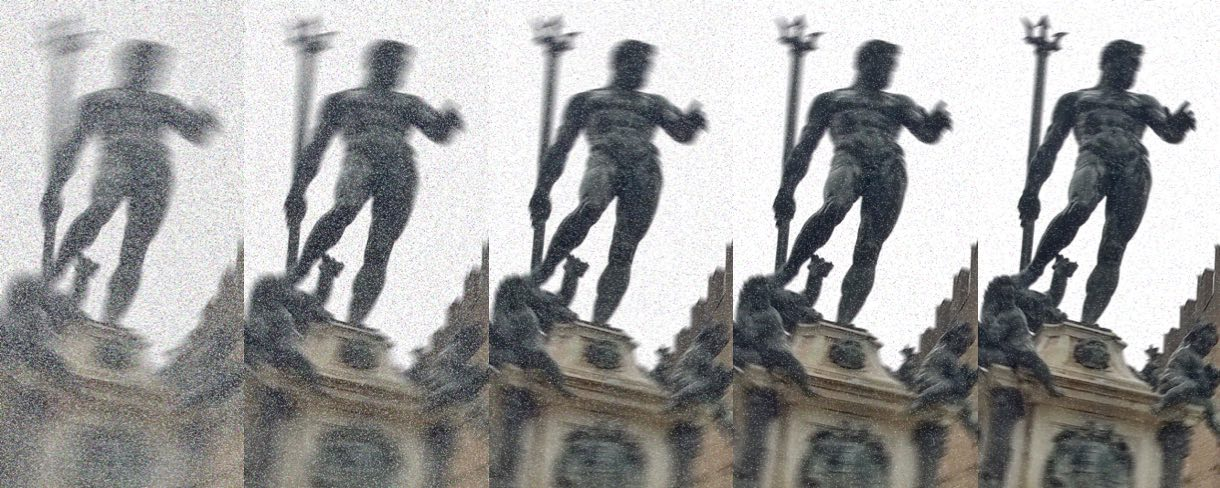
\includegraphics[width=\paperwidth]{images/nettuni_small}}; % Background
    \draw[anchor=north] (midpoint) node [fill=blue!30!white,fill opacity=0.6,text opacity=1,inner sep=1cm]{\Huge\centering\bfseries\sffamily\parbox[c][][t]{\paperwidth}{\centering SIAM Conference\\on\\IMAGING SCIENCE\\ Program\\[15pt] % Book title
    {\Large June 5-8, 2018}\\[20pt] % Subtitle
    {\huge University of Bologna\\Bologna, Italy}}}; % Author name
  \end{tikzpicture}};
\end{tikzpicture}
\vfill
\endgroup



%----------------------------------------------------------------------------------------
%	CONFERENCE THEMES
%----------------------------------------------------------------------------------------

\newpage
~\vfill
\thispagestyle{empty}

\noindent \textsc{https://siam-is18.dm.unibo.it}

\bigskip

\noindent This conference is the biennial activity of the SIAM Activity Group on Imaging Science.

\vspace{0.5cm}

\noindent The SIAM Activity Group on Imaging Science brings together SIAM members and other scientists and engineers with an interest 
in the mathematical and computational aspects of imaging.
The activity group organizes the biennial SIAM Conference on Imaging Science, awards the SIAG/IS Best Paper Prize
every two years to the authors of the best paper on mathematical and computational aspects of imaging, awards the SIAG/IS 
Early Career Prize to an outstanding early career researcher in the field of imaging science, and maintains a wiki, a
member directory, and an electronic mailing list.

\newpage

\section*{Conference Themes}

Reconstruction, enhancement, segmentation, analysis, registration, compression, representation, tomography, machine learning and tracking of two and three dimensional images are vital to many areas of science, medicine, and engineering. The increasingly sophisticated mathematical, statistical and computational methods employed in these research areas are referred to as \emph{Imaging Science}.\\ 
These techniques include transform and orthogonal series methods, nonlinear optimization, numerical linear algebra, integral equations, partial differential equations, Bayesian and other statistical inverse estimation methods, operator theory, differential geometry, information theory, interpolation and approximation, inverse problems, computer graphics and vision, stochastic processes, and others.

\smallskip

SIAM-IS18 will exchange research results and address open issues in all aspects of imaging science
and provide a forum for the presentation of work in imaging science.



\section*{Committee}

\bigskip
\noindent \textbf{\color{siamblue}General Co-Chairs}
\bigskip

\begin{itemize}
  \item[] \member{Omar Ghattas}{University of Texas at Austin, USA}
  \item[] \member{Fiorella Sgallari}{University of Bologna}
\end{itemize}

\bigskip
\noindent \textbf{\color{siamblue}Scientific Committee}
\bigskip

\begin{itemize}
  \item[] \member{Marcelo Bertalm\'io}{University Pompeu Fabra, Spain}
  \item[] \member{Julianne Chung}{Virginia Tech., USA}
  \item[] \member{Per Christian Hansen}{Technical University of Denmark, Denmark }
  \item[] \member{Jari Kaipio}{University of Auckland, New Zealand}
  \item[] \member{Eric Miller}{Tufts University, USA}
  \item[] \member{Mila Nikolova}{CNRS ENS Cachan, France}
  \item[] \member{Ronny Ramlau}{Kepler University Linz, Austria and Johann Radon Institute, Austria}
  \item[] \member{Carola Sch\"{o}nlieb}{University of Cambridge, United Kingdom}
  \item[] \member{Gabriele Steidl}{Tech.Univ. Kaiserslautern, Germany}
  \item[] \member{Xue-Cheng Tai}{Hong Kong Baptist University, China }
  \item[] \member{Laura Waller}{University of California Berkeley, USA }
  \item[] \member{Brendt Wohlberg}{Los Alamos National Laboratory, USA}
\end{itemize}

\bigskip
\noindent\textbf{\color{siamblue}Organizing Committee}
\bigskip

\begin{itemize}
  \item[] \member{Carolina Beccari}{Dept. Mathematics, University of Bologna}
  \item[] \member{Giulio Casciola}{Dept. Mathematics, University of Bologna}
  \item[] \member{Salvatore Cuomo}{Dept. Mathematics and Applications ``Renato Caccioppoli'', University of Naples}
  \item[] \member{Luigi Di Stefano}{Dept. Computer Science and Engineering, University of Bologna}
  \item[] \member{Giovanni Dore}{Dept. Mathematics, University of Bologna}
  \item[] \member{Maurizio Falcone}{Dept. Mathematics, University of Roma ``La Sapienza''}
  \item[] \member{Luca Formaggia}{Department of Mathematics, Politecnico di Milano}
  \item[] \member{Patrizio Frosini}{Dept. Mathematics, University of Bologna}
  \item[] \member{Germana Landi,}{Dept. Mathematics, University of Bologna}
  \item[] \member{Alessandro Lanza}{Dept. Mathematics, University of Bologna}
  \item[] \member{Damiana Lazzaro}{Dept. Mathematics, University of Bologna}
  \item[] \member{Roberto Mecca}{University of Bologna and University of Cambridge}
  \item[] \member{Serena Morigi}{Dept. Mathematics, University of Bologna}
  \item[] \member{Michele Piana}{Dept. Mathematics, University of Genova}
  \item[] \member{Elena Loli Piccolomini}{Dept. Mathematics, University of Bologna}
  \item[] \member{Giulia Scalet}{Dept. Civil Engineering and Architecture, University of Pavia}
  \item[] \member{Federica Sciacchitano}{Dept. Mathematics, University of Genova}
  \item[] \member{Valeria Simoncini}{Dept. Mathematics, University of Bologna}
  \item[] \member{Giulia Spaletta}{Dept. Mathematics, University of Bologna}
  \item[] \member{Fabiana Zama}{Dept. Mathematics, University of Bologna}
\end{itemize}



\usechapterimagetrue
\chapterimage{images/nettuni_small} 
\pagestyle{empty} % No headers

\tableofcontents % Print the table of contents itself
\cleardoublepage % Forces the first chapter to start on an odd page so it's on the right
\pagestyle{fancy} % Print headers again

\newpage
\section*{Program At-A-Glance}
\addcontentsline{toc}{section}{Program AT-A-Glance}

\part{General Information}
\chapterimage{images/nettuni_small} 
\chapter*{General Information}
\newpage

%-----Registration Desk
\gisection{Registration Desk}
\addcontentsline{toc}{section}{Registration Desk}
The registration desk is located in the hall of Building A (via B. Andreatta 8) and is open during the following hours:

\bigskip

\begin{itemize}
  \item[] Monday, June 4: 3:00 PM - 6:30 PM
  \item[] Tuesday, June 5: 11:30 AM - 6:30 PM
  \item[] Wednesday, June 6: 8:00 AM - 6:30 PM
  \item[] Thursday, June 7: 8:00 AM - 1:30 PM
  \item[] Friday, June 8: 8:00 AM - 1:30 PM
\end{itemize}

%-----Badges
\gisection{Badges} 
Carry your badge during the conference so that you can be admitted to all technical sessions, coffee breaks, lunches, reception and banquet.\\
\textbf{Emergency numbers} are provided on the back of your name badge! 

%-----Registration Fee Includes
\gisection{Registration Fee Includes}

\bigskip

\begin{itemize}
  \item Admission to all technical sessions
  \item Business Meeting (open to SIAG/IS members)
  \item Social dinner (Wednesday)
  \item Coffee breaks 
  \item Welcome lunch (Tuesday)
  \item Welcome cocktail during the evening Poster Session (Tuesday)
  \item Room set-ups and audio/visual equipment
  \item Wi-Fi access at the conference
\end{itemize}%-----Conference Talk Arrangements

%-----Conference Talk Arrangements

\gisection{Conference Talk Arrangements}

\noindent All \textbf{plenary talks} will have a slot of 45 minutes
(5 minutes reserved for questions and discussion included).\\\\
The \textbf{minitutorials} will last 2 hours.\\\\
All \textbf{minisymposia talks} will have a slot of 30 minutes (5 minutes reserved for questions and discussion included).\\
All \textbf{contributed talks} will last 20 minutes (5 minutes reserved for questions and discussion included).\\\\
If you need to copy your presentation slides from your USB to a computer in lecture hall or meeting room, please do it in advance before
the session starts.

%-----Important Notice to Poster Presenters
\gisection{Important Notice to Poster Presenters}

\noindent The \textbf{poster sessions} are scheduled:
\begin{center}
  \textbf{Tuesday, June 5} \\
  from 6:30 PM onwards \\
  in Building A and B\\
  with Welcome cocktail

  \bigskip
   
  \textbf{Wednesday, June 6} \\
  from 11:30 AM to 1:00 PM \\
  in Building A and B
\end{center}

\noindent The \textbf{Best Poster Award} will be given on Friday, June 8 at 1:00 PM in Building A, Room A.\\

\noindent All posters participating to the Best Poster Award are available on the Conference website from June 1.\\
Poster presenters are requested to set up
their material on the provided poster boards (70 cm x 100 cm), following the instructions in the participant folder and be present during both sessions.  
All materials must be posted by Tuesday, June 5 at 6:00 PM.
The conference is not responsible for discarded posters.

%------------Wi-Fi Access
\gisection{Wi-Fi Access}
The username and password of your account during the conference period (5-8 June) can be found in your folder.

%-------------------Standard Audio/VIsual Set-Up in Meeting Rooms
\gisection{Standard Audio/Visual Set-Up in Meeting Rooms}
The plenary session room has a PC, two screens and two data projectors.\\ 
All other concurrent/breakout rooms have a PC, a screen, a data projector and a whiteboard (overhead projectors are also available).\\
The data projectors support VGA connection only. Presenters requiring an HDMI or alternate connection must provide their own adaptor.\\
Cables or adaptors for Apple computers are not supplied, as they vary for each model: please bring your own cable/adaptor if using a Mac computer. 
The conference is not responsible for the safety and security of speakers' computers.

%-------------Recording of presentations
\gisection{Presentations Recording}
During the conference audio and video recording is prohibited without the written permission of the speaker and the conference organizers.

%-------------SIAM Books and Journal
\gisection{SIAM Books and Journals}
%Display copies of books and complimentary copies of journals are available on site. SIAM books are available at a discounted price during the conference. The book booth will be staffed from 9:00 AM through 6:00 PM. \\If a SIAM books representative is temporarily away from the booth, completed order forms and payment (credit cards are preferred) may be taken to the registration desk. The books table will close at 4:00 PM on Friday??? (2016)\\
%Completed order forms should be emailed or faxed to the SIAM office directly. It is not allowed to carry out on site transaction during the conference period??? (2014)


\noindent Display copies of selected SIAM books are available on site.

\bigskip

\noindent SIAM books are offered at \textbf{discounted prices} for all attendees. 
SIAM members can apply their member discount, and all attendees are entitled to a 20\% Conference Discount.

\bigskip

\noindent The SIAM \textbf{book table} will be staffed from 9:00 AM through 5:30 PM. 
The book table will close at 4:00 PM on Friday. 
If the SIAM book table is temporarily unattended, please take a copy of the Titles on Display to order online and receive the Conference Discount. 
\textit{(Note: all prices in the Titles on Display are in Euros.)}

\gisection{Table Top Displays}

\begin{itemize}
  \item SIAM: Building A, second floor
  \item IOP: Buiding A, first floor
  \item Springer Nature: Building A, first floor
\end{itemize}

%------------------ GET TOGETHERS
\addcontentsline{toc}{section}{Get-togethers}
\gisection{Get-togethers}

\subsection*{Tuesday, June 5}

\begin{itemize}
  \item[] 11:45 AM - 1:30 PM, Welcome lunch
  \item[] 6:30 PM - 8:30 PM, Poster Session I and Welcome cocktail
\end{itemize}

\subsection*{Wednesday, June 6}

\begin{itemize}
  \item[] 11:30 AM - 1:00 PM, Poster Session II
  \item[] 5:45 PM - 6:30 PM Business Meeting (open to SIAG/IS members)
  \item[] 8:00 PM Social dinner
\end{itemize}

%---------------Lunches
\newpage % PIETRO FIXME
\gisection{Lunches}
There are multiple options for your lunches on Wednesday, Thursday and Friday. 
\bigskip
\begin{itemize}
  \item Two different \textbf{lunch boxes} prepared by the catering in the conference location: it can be ordered at the coffee desk the day before.
  \item The John Hopkins University canteen in front of the conference location: Please show your conference badge.
  \item Elior canteen, Piazza Vittorio Puntoni 1: Special rates for the conference participants.
\end{itemize}
\bigskip
Several bars and restaurants are available for lunch in the area surrounding via Andreatta and via Belmeloro: The complete list is in your folder.

%---------------Conference Banquet
\gisection{Conference Banquets}
The \textbf{Conference banquet} will be served in Palazzo Re Enzo, in Piazza del Nettuno 1C: Please carry your badge and ticket with you for admission. For security
reasons, only 650 persons are admitted. So a second \textbf{special dinner} is organized in the same evening at Cantina Bentivoglio, via Mascarella 4 with 
Jazz music.

\bigskip 

\noindent Additional conference banquet \textbf{tickets} are available at the price of 65 euros. 
Please purchase it at the registration desk before Tuesday, June 5 afternoon.\\

%---------------Child Care
\gisection{Child Care}
\subsection*{Le cicogne} 
Typical rates: if reserved a few days in advance: \euro 16 / each hour (for a maximum of 2-3-4 hours) for a basic baby sitting and \euro 20/each hour for a baby sitter speaking foreign languages.
If requested one day before: \euro 18 + hourly rate.
If requested the same day: \euro 28 + hourly rate.

\smallskip\noindent website: \href{http://www.lecicogne.net}{http://www.lecicogne.net}

\subsection*{Born to life}
Typical rates: \euro 25 agency fee + hourly rate \euro 13. After 10 PM: \euro 15 Foreign languages available. Reservations: 2 weeks in advance.

\smallskip\noindent website: \href{http://www.bolognababysitter.it}{http://www.bolognababysitter.it}

\gisection{General information in Bologna}

\begin{itemize}
  \item Emergency Phone Number: 118 Medical Emergencies; 113 Emergency Police Help Number; 115 Fire Department; 
  \item Time Zone: CEST (Central European Summer Time); UTC/GMT+2
  \item Electricity: 220 V, 50Hz; power sockets follow European standards
  \item Currency: Euro (EUR)
  \item Dial Country Code: +39
  \item Working hours:Banks: 8:30 AM - 1:30 PM; 2:30 PM - 3:45 PM (Monday to Friday) 
  \item Buses in Bologna: visit https://www.tper.it/ 
  \item Pharmacies: 09:00 AM - 1:00 PM, 3:30 PM - 7:30 PM (Monday to Saturday, some are open 24 hours a day, everyday) 
  \item Shops: 9:30 AM - 1:00 PM; 3:30PM - 7:30 (Monday to Saturday) 
  \item Bologna Touristic Bureau: https://www.bolognawelcome.com/en/
\end{itemize}

%---------------Please Note
\gisection{Please note}
The conference is not responsible for the safety and security of participants' computers. Do not leave your laptop computers and personal belongings unattended. Please remember to turn off your mobile during all the sessions.\\\\ The conference cannot provide photocopying and dollar exchange service. A bank can be found in piazza Aldrovandi 12/A (opening hours: 8:20 AM-1:20 PM and 2:30 PM-4:00 PM).

%---------------Comments
\gisection{Comments?}
Comments about SIAM IS18 are encouraged! Please send it to Cynthia Phillips, SIAM Vice President for Programs (vpp@siam.org).

\newpage
\addcontentsline{toc}{section}{Sponsors and Exhibitors}

\setlength{\columnseprule}{0pt}
\begin{center}

\section*{\color{siamblue}{ORGANIZED BY}}
\vspace{0.1cm}

\begin{multicols}{4}
\includegraphics[width=3.3cm]{images/sponsors/unibo}    
\includegraphics[width=3.3cm]{images/sponsors/siam_logo} 
\end{multicols}

\section*{\color{siamblue}{IN COOPERATION WITH}}
\vspace{0.1cm}

\begin{multicols}{4}
\includegraphics[width=5.0cm]{images/sponsors/ieee} 
\includegraphics[width=3.0cm]{images/sponsors/Ohne_Schriftzug} 
\includegraphics[width=3.2cm]{images/sponsors/simai}
\end{multicols}

\section*{\color{siamblue}{SPONSOR}}
\vspace{0.1cm}

\begin{multicols}{4}
\includegraphics[width=3.6cm]{images/sponsors/apt}    
\includegraphics[width=3.1cm]{images/sponsors/cineca} 
\includegraphics[width=3.1cm]{images/sponsors/bper}
\includegraphics[width=3.6cm]{images/sponsors/datalogic}
\end{multicols}

\begin{multicols}{4}
\includegraphics[width=3.5cm]{images/sponsors/comunico_italiano} 
\includegraphics[width=3.5cm]{images/sponsors/napoli} 
\includegraphics[width=3.5cm]{images/sponsors/azimut}
\includegraphics[width=3.3cm]{images/sponsors/gncs}
\end{multicols}

\begin{multicols}{4}
\includegraphics[width=3.3cm]{images/sponsors/arces} 
\includegraphics[width=3.3cm]{images/sponsors/tsc} 
\includegraphics[width=3.3cm]{images/sponsors/felsineo}
\includegraphics[width=4.6cm]{images/sponsors/rotary}
\end{multicols}

\begin{multicols}{4}
\includegraphics[width=3.1cm]{images/sponsors/rotaract} 
\end{multicols}

\section*{\color{siamblue}{UNDER THE PATRONAGE OF}}
\vspace{0.1cm}

\begin{multicols}{4}
\includegraphics[width=3.0cm]{images/sponsors/regione_emilia_romagna}
\includegraphics[width=3.0cm]{images/sponsors/comune_bologna}
\includegraphics[width=3.0cm]{images/sponsors/accademiascienzebologna}
\includegraphics[width=3.0cm]{images/sponsors/ordine_ingegneri}
\end{multicols}

\end{center}
\setlength{\columnseprule}{0.5pt}




\chapterimage{images/nettuni_small} 
\addcontentsline{toc}{section}{Plenary Talks and Biographies}
\chapter*{Plenary Talks and Biographies}
\begin{center}
  \plenaryitem{Tuesday, 5}{9:45 -- 10:30}{IP1: Flexible methodology for image segmentation}{Raymond H. Chan}{Department of Mathematics, The Chinese University of Hong Kong,  Hong Kong}
  
  \plenaryitem{Tuesday, 5}{10:30 -- 11:15}{IP2: The expanding role of inverse problems in informing climate science and policy}{Anna Michalak}{Department of Global Ecology, Carnegie Institution for Science, Stanford, USA}

  \plenaryitem{Wednesday, 6}{8:15 -- 9:00}{IP3: Fake ID documents and counterfeited products: overview of image analysis techniques to fight them}{Clarisse Mandridake}{Surys Group, France}

  \plenaryitem{Thursday, 7}{8:15 -- 9:00}{IP4: Fast analog to digital compression for high resolution imaging}{Yonina Eldar}{Department of EE Technion, Israel Institute of Technology, Haifa, Israel}

  \plenaryitem{Thursday, 7}{13:00 -- 13:45}{IP5: Image Segmentation and Understanding: A Challenge for Mathematicians}{Christoph Schn\"{o}rr}{Institute of Applied Mathematics, University of Heidelberg, Germany}

  \plenaryitem{Friday, 8}{8:15 -- 9:00}{IP6: Linearly-convergent stochastic gradient algorithms}{Francis Bach}{Departement d'Informatique de l'Ecole Normale Superieure Centre de Recherche INRIA de Paris, France}
\end{center}

\vfill

\noindent{Invited Plenary Presentations  IP1 and IP2 will take place in Aula Magna Santa Lucia, while the other Invited Presentations will take place in Building A, Room A and Room B in via Andreatta, 8.}

%----------------INVITED PLENARY PRESENTATIONS
{\small{Invited Plenary Presentations  IP1 and IP2 on Tuesday, June 5, will take place in Aula Santa Lucia, while the other Invited Presentation will take place in Building A, Rooms A and B in via Belmeloro 14}}
%\vspace{2cm}
%---IP1
\newpage\vspace{2cm}
\begin{center}{\Large{
Tuesday, June 5, 9:45 AM - 10:30 AM \\
\textbf{IP1: Linearly-convergent stochastic gradient algorithms}\\
Francis Bach, Departement d'Informatique de l'Ecole Normale Superieure Centre de Recherche INRIA de Paris, PARIS, France}}
\end{center}
\vspace{1cm}

\begin{wrapfloat}{figure}{o}{0pt}
\includegraphics[scale=1.25]{Francis_Bach.jpg}
\end{wrapfloat}

Francis Bach is a researcher at Inria, leading since 2011 the machine learning project-team, which is part of the Computer Science Department at Ecole Normale Sup\'erieure. He graduated from Ecole Polytechnique in 1997 and completed his Ph.D. in Computer Science at U.C. Berkeley in 2005, working with Professor Michael Jordan. He spent two years in the Mathematical Morphology group at Ecole des Mines de Paris, then he joined the computer vision project-team at Inria/Ecole Normale Sup\'erieure from 2007 to 2010. Francis Bach is primarily interested in machine learning, and especially in graphical models, sparse methods, kernel-based learning, large-scale convex optimization, computer vision and signal processing. He obtained in 2009 a Starting Grant and in 2016 a Consolidator Grant from the European Research Council, and received in 2012 the Inria young researcher prize. In 2015, he was program co-chair of the International Conference in Machine learning (ICML).\\\\

\textbf{Abstract:}\\

Many machine learning and signal processing problems are traditionally cast as convex optimization problems where the objective function is a sum of many simple terms. In this situation, batch algorithms compute gradients of the objective function by summing all individual gradients at every iteration and exhibit a linear convergence rate for strongly-convex problems. Stochastic methods rather select a single function at random at every iteration, classically leading to cheaper iterations but with a convergence rate which decays only as the inverse of the number of iterations. In this talk, I will present the stochastic averaged gradient (SAG) algorithm which is dedicated to minimizing finite sums of smooth functions; it has a linear convergence rate for strongly-convex problems, but with an iteration cost similar to stochastic gradient descent, thus leading to faster convergence for machine learning and signal processing problems. I will also mention several extensions, in particular to saddle-point problems, showing that this new class of incremental algorithms applies more generally.



%---IP2
\newpage\vspace{2cm}
\begin{center}{\Large{
Tuesday, June 5, 10:45 AM - 11:30 AM \\
\textbf{IP2: Flexible methodology for image segmentation}\\
Raymond H. Chan, Department of Mathematics, The Chinese University of Hong Kong,  Hong Kong}}
\end{center}
\vspace{1cm}

\begin{wrapfloat}{figure}{o}{0pt}
\includegraphics[scale=0.75]{Raymond_Chan.jpg}
\end{wrapfloat}

Raymond Chan obtained his PhD degree from The Courant Institute of Mathematical Sciences in 1985. He is now the Chairman of the Mathematics Department at The Chinese University of Hong Kong. He won a Leslie Fox Prize in 1989; a Feng Kang Prize in 1997; a Morningside Award in 1998; and 2011 Higher Education Outstanding Scientific Research Output Awards from the Ministry of Education in China. He was elected a SIAM Fellow in 2013. He has published 120 journal papers and has been in the ISI Science Citation List of Top 250 Highly-Cited Mathematicians in the world since 2004. Chan has served on the editorial boards of many journals, including: Journal of Mathematical Imaging and Vision, Journal of Scientific Computing, Numerical Linear Algebra with Applications, SIAM Journal on Imaging Sciences, and SIAM Journal on Scientific Computing. 

%---IP3
\newpage\vspace{2cm}
\begin{center}{\Large{
Wednesday, June 6, 8:30 AM - 9:15 AM \\
\textbf{IP3: Fast analog to digital compression for high resolution imaging}\\
Yonina Eldar, Department of EE Technion, Israel Institute of Technology, Haifa, Israel
}}\end{center}
\vspace{1cm}


\begin{wrapfloat}{figure}{o}{0pt}
\includegraphics[scale=0.05]{Yonina_Eldar_small2}
\end{wrapfloat}
Yonina C. Eldar is a Professor in the Department of Electrical Engineering at the Technion, Israel Institute of Technology, Haifa, where she holds the Edwards Chair in Engineering. 
She is also a Research Affiliate with the Research Laboratory of Electronics at MIT and a Visiting Professor at Duke University, and was a Visiting Professor at Stanford University. 
She received the B.Sc. degree in physics and the B.Sc. degree in electrical engineering both from Tel-Aviv University (TAU), Tel-Aviv, Israel, in 1995 and 1996, respectively, and the Ph.D. degree in electrical engineering and computer science from the Massachusetts Institute of Technology (MIT), Cambridge, in 2002.
She has received many awards for excellence in research and teaching, as
the IEEE Signal Processing Society Technical Achievement Award (2013), the IEEE/AESS Fred Nathanson Memorial Radar Award (2014) and the IEEE Kiyo Tomiyasu Award (2016).
She was a Horev Fellow of the Leaders in Science and Technology program at the Technion and an Alon Fellow. 
She received the Michael Bruno Memorial Award from the Rothschild Foundation, the Weizmann Prize for Exact Sciences, the Wolf Foundation Krill Prize for Excellence in Scientific Research, the Henry Taub Prize for Excellence in Research (twice), the Hershel Rich Innovation Award (three times), the Award for Women with Distinguished Contributions, the Andre and Bella Meyer Lectureship, the Career Development Chair at the Technion, the Muriel \& David Jacknow Award for Excellence in Teaching, and the Technion's Award for Excellence in Teaching (two times). 
She received several best paper awards and best demo awards together with her research students and colleagues and was selected as one of the 50 most influential women in Israel.
She is the Editor in Chief of Foundations and Trends in Signal Processing, a member of several IEEE Technical Committees and Award Committees, an IEEE Fellow, and a EURASIP Fellow.
She is also a member of the Young Israel Academy of Science and was a member of the Israel Committee for Higher Education.\\\\
\textbf{Abstract:}\\
The famous Shannon-Nyquist theorem has become a landmark in the development of digital signal processing. However, in many modern applications, the signal bandwidths have increased tremendously, while the acquisition capabilities have not scaled sufficiently fast. Consequently, conversion to digital has become a serious bottleneck. Furthermore, the resulting high rate digital data requires storage, communication and processing at very high rates which is computationally expensive and requires large amounts of power. In the context of medical imaging sampling at high rates often translates to high radiation dosages, increased scanning times, bulky medical devices, and limited resolution. In this talk, we present a framework for sampling and processing a wide class of wideband analog signals at rates far below Nyquist by exploiting signal structure and the processing task and show several demos of real-time sub-Nyquist prototypes. We then consider applications of these ideas to a variety of problems in medical and optical imaging including fast and quantitative MRI, wireless ultrasound, fast Doppler imaging, and correlation based super-resolution in microscopy and ultrasound which combines high spatial resolution with short integration time. We end by discussing several modern methods for structure-based phase retrieval which has applications in several areas of optical imaging.

%--IP4
\newpage\vspace{2cm}
\begin{center}{\Large{
Wednesday, June 6, 1:30 PM - 2:15 PM \\
\textbf{IP4: Fake ID documents and counterfeited products: overview of image analysis techniques to fight them}\\
Clarissa Mandridake, Surys Group, France}}
\end{center}
\vspace{1cm}

\begin{wrapfloat}{figure}{o}{0pt}
\includegraphics[scale=0.12]{Clarissa_Mandridake.jpg}
\end{wrapfloat}
Mrs Clarisse Manjary Mandridake received his PhD in Image and Signal Processing from the University of Bordeaux I, France, for her works on bi-dimensional signal decomposition applied to classification of textured images, done in Laboratoire Automatique Productique et Traitement du Signal, and in closed connection with ARIANA Project in INRIA Sophia-Antipolis. She joined the research team of Advestigo for her postdoc year in 2002. As a researcher at Advestigo and later at Hologram Industries (now renamed SURYS), she developed technologies for the representation, indexation and search of images and videos in large scale databases. She is now in charge of the coordination of the research project for the SURYS digital labs and animates the scientist partnerships with University labs. Her expertise covers Applied Mathematics, image characterization, fingerprinting and authentication on various physical supports, from ID documents to smartlabels. More recently, his area of interest is to contribute to technological innovation for use by poor countries or developing countries in order to help them put in place what is called "good governance". It is a sine qua non Condition for any future economic development.


%--IP5
\newpage\vspace{2cm}
\begin{center}{\Large{
Thursday, June 7, 1:30 PM - 2:15 PM \\
\textbf{IP5: The expanding role of inverse problems in informing climate science and policy}\\
Anna Michalak, Department of Global Ecology, Carnegie Institution for Science, Stanford, CA, USA}}
\end{center}
\vspace{1cm}

\begin{wrapfloat}{figure}{o}{0pt}
\includegraphics[scale=0.065]{Anna_Michalak_small}
\end{wrapfloat}
Dr. Anna M. Michalak is a faculty member in the Department of Global Ecology of the Carnegie Institution for Science in Stanford, California, and an Associate Professor in the Department of Earth System Science at Stanford University. Prior to joining Carnegie, she was the Frank and Brooke Transue Faculty Scholar and Associate Professor at the University of Michigan, Ann Arbor. Her research interests primarily lie in two areas. She explores the impacts of climate change and extreme events on freshwater and coastal water quality via influences on nutrient delivery to, and on conditions within, water bodies. She also studies the cycling and emissions of greenhouse gases at the Earth surface at regional to global scales ? scales directly relevant to informing climate science and policy ? primarily through the use of atmospheric observations that provide the clearest constraints at these critical scales. She is the recipient of numerous awards, including the Presidential Early Career Award for Scientists and Engineers (nominated by NASA), the NSF CAREER award, the Association of Environmental Engineering and Science Professors Outstanding Educator Award, and the Leopold Fellowship in environmental leadership. Dr. Michalak holds a B.Sc. from the University of Guelph, Canada, and M.S. and Ph.D. degrees from Stanford.

%--IP6
\newpage\vspace{2cm}
\begin{center}{\Large{
Friday, June 8, 1:30 PM - 2:15 PM \\
\textbf{IP6: Image Segmentation and Understanding: A Challenge for Mathematicians}\\
Christoph Schn\"{o}rr, Institute of Applied Mathematics, University of Heidelberg, Germany}}
\end{center}
\vspace{1cm}

\begin{wrapfloat}{figure}{o}{0pt}
\includegraphics[scale=0.25]{Schnoerr_small}
\end{wrapfloat}
Christoph Schn\"{o}rr received his degrees from the Technical University of Karlsruhe (today: Karlsruhe Institute of Technology) and the University of Hamburg, respectively. He worked as a researcher at the Fraunhofer Institut of Information and Data Processing in Karlsruhe before moving to the University of Hamburg. In 1998, he became full professor at the University of Mannheim, where he set up and directed the Computer Vision and Pattern Recognition Group. He moved to the Heidelberg University in 2008 where he is heading the Image and Pattern Analysis Group at the Institute of Applied Mathematics, which also is member of the Interdisciplinary Center for Scientific Computing.

Christoph Schn\"{o}rr has been coordinating 2010-2018 a research training group focusing on probabilistic graphical models and its applications to image analysis, funded by the German Science Foundation. He is one of 4 directors of the Heidelberg Collaboratory for Image Processing that implements and explores novel ways of combining basic strategic research in academia and research labs in industry, as part of the excellence initiative of the Heidelberg University. He served 2005-2014 as co-editor in chief of the International Journal of Computer Vision and currently as associate editor for the Journal of Mathematical Imaging and Vision and the SIAM Journal of Imaging Science.

His research interests include mathematical models of image analysis and numerical optimisation.


\chapterimage{images/nettuni_small} 
\addcontentsline{toc}{section}{Minitutorials and Biograpies}
\chapter*{Minitutorials and Biograpies}
\begin{flushright}All minitutorials will take place in Building A, Room B in via Andreatta, 8.\end{flushright}

\begin{center}
  \plenaryitem{Wednesday, 6}{ 9:30 -- 11:30 }{MT1: Computational Uncertainty Quantification for Inverse Problems}{John Bardsley}{Department of Mathematical Sciences, The University of Montana, USA}

  \plenaryitem{Thursday, 7}{ 9:30 -- 11:30 }{MT2: Regularization of Inverse Problem}{Otmar Scherzer}{Computational Science Center, University of Vienna, Austria}

  \plenaryitem{Friday, 8}{ 9:30 -- 11:30 }{MT3: Automated 3D reconstruction from satellite images}{Gabriele Facciolo}{Centre de math\'ematiques et de leurs applications [CMLA] - \'Ecole Normale Sup\'erieure Paris-Saclay, France \newline with Carlo de Franchis and Enric Meinhardt-Llopis (\'Ecole Normale Sup\'erieure Paris-Saclay, France)}
\end{center}


%--------------MINITUTORIALS
\newpage
\chapter*{Minitutorials and Biography}
\addcontentsline{toc}{section}{Minitutorials and Biography}

\begin{center}\textbf{Wednesday, June 6, \\9:30 AM - 11:30 AM \\Room B}\end{center}
\begin{center}
\textbf{MT1: Computational Uncertainty Quantification for Inverse Problems}\\
Organizer: John Bardsley, Department of Mathematical Sciences, The University of Montana, MT, USA
\end{center}

\vspace{1cm}
\begin{center}\textbf{Thursday, June 7, \\9:30 AM - 11:30 AM \\Room B}\end{center}
%\vspace{2cm}
\begin{center}
\textbf{MT2: Automated 3D reconstruction from satellite images}\\
Organizer: Gabriele Facciolo, Centre de math\'ematiques et de leurs applications [CMLA] - Ecole Normale Sup\'erieure de Cachan, France\\
with\\ Carlo de Franchis and Enric Meinhardt-Lopis - Ecole Normale Sup\'erieure de Cachan, France
\end{center}
\vspace{1cm}
\begin{center}\textbf{Friday, June 8, \\9:30 AM - 11:30 AM \\Room B}\end{center}
%\vspace{2cm}
\begin{center}
\textbf{MT3: Regularization of Inverse Problem}\\
Organizer: Otmar Scherzer, Computational Science Center, University of Vienna, Austria
\end{center}

\newpage
%---------MT1
\begin{center}\textbf{Wednesday, June 6, 9:30 AM - 11:30 AM, Room B}\end{center}
%\vspace{2cm}
\begin{center}
\textbf{MT1: Computational Uncertainty Quantification for Inverse Problems}\\
Organizer: John Bardsley, Department of Mathematical Sciences, The University of Montana, MT, USA
\end{center}
%\vspace{2cm}

\begin{wrapfloat}{figure}{o}{0pt}
\includegraphics[scale=0.98]{John_Bardsley.jpg}
\end{wrapfloat}
Dr. Johnathan M. Bardsley is Professor of Mathematics at the University of Montana (UM) in Missoula, Montana, USA. He received his PhD from Montana State University in 2002 under the direction of Professor Curtis R. Vogel, with a dissertation focused on computational inverse problems. He then spent one year as a post-doc at the Statistical and Applied Mathematical Sciences Institute, under the direction of Professor H. Thomas Banks. He began his current job at UM in 2003, and since then has spent two years abroad as a visiting Professor: first at the University of Helsinki in Finland in 2006-07; and then at the University of Otago in New Zealand in 2010-11. Dr. Bardsley has published over 45 refereed journal articles and has given many presentations on his research around the world. He also organized Montana Uncertainty Quantification, a conference/workshop that took place at UM in June 2015. Dr. Bardsley's current research is focused, broadly, on uncertainty quantification for inverse problems, and more specifically, on the development of Markov chain Monte Carlo methods for sampling from posterior distributions that arise in both linear and nonlinear inverse problems. He has a forthcoming book, titled Computational Methods and Uncertainty Quantification for Inverse Problems, that will be published by SIAM.\\

\textbf{Abstract:} 
The field of inverse problems is fertile ground for the development of computational uncertainty quantification methods. This is due to the fact that, on the one hand, inverse problems involve noisy measurements, leading naturally to statistical (and hence uncertainty) estimation problems. On the other hand, inverse problems involve physical models that, upon discretization, are known only up to a high-dimensional vector of parameters, making them computationally challenging. Estimating a high-dimensional parameter vector in a discretized physical model from measurements of model output defines computational inverse problems. Such problems are typically unstable in that the estimates don?t depend continuously on the measurements. Regularization is a technique that provides stability for inverse problems, and in the Bayesian setting, it is synonymous with the choice of the prior probability density function. Once a prior is chosen, the posterior probability density function results, and it is the solution of the inverse problem in the Bayesian setting. The posterior maximizer ? known as the MAP estimator ? provides a stable estimate of the unknown parameters. However, uncertainty quantification requires that we extract more information from the posterior, which often requires sampling. The posterior density functions that arise in typical inverse problems are high-dimensional, and are often non-Gaussian, making the corresponding sampling problems challenging. In this mini-tutorial, I will begin with a discussion of inverse problems, move on to Bayesian statistics and prior modeling using Markov random fields, and then end with a discussion of some Markov chain Monte Carlo methods for sampling from posterior density functions that arise in inverse problems. 


%----MT2
\vspace{2cm}
\begin{center}\textbf{Thursday, June 7, 9:30 AM - 11:30 AM, Room B}\end{center}
%\vspace{2cm}
\begin{center}
\textbf{MT2: Automated 3D reconstruction from satellite images}\\
Organizer: Gabriele Facciolo, Centre de math\'ematiques et de leurs applications [CMLA] - Ecole Normale Sup\'erieure de Cachan, France\\
with\\ Carlo de Franchis and Enric Meinhardt-Lopis - Ecole Normale Sup\'erieure de Cachan, France
\end{center}

%\vspace{2cm}
\begin{wrapfloat}{figure}{o}{0pt}
\includegraphics[scale=0.4]{gabriele_facciolo.jpg}
\end{wrapfloat}
Gabriele Facciolo received his B.Sc. and M.Sc. in computer science from Universidad de la Republica del Uruguay, and his Ph.D. (2011) from Universitat Pompeu Fabra under the supervision of Vicent Caselles. During his thesis he contributed to a pioneering mathematical formalization of the image inpainting problem, and a formulation of temporally consistent video editing robust to illumination changes. He joined Jean-Michel Morel's group at the \'{E}cole Normale Sup\'erieure Paris-Saclay in 2011 where he is currently associate research professor. He has participated in many industrial projects, creating image processing algorithms and transferring technology with the CNES, Schlumberger, DxO Labs, and the foundation BarcelonaMedia. He has more than ten years of experience designing algorithms for remote sensing applications and collaborating with the French Space Agency (CNES) as part of the MISS project (Mat\'ematiques de l'Imagerie St\'er\'eoscopique Spatiale). The 3D reconstruction algorithms and the satellite stereo pipeline (github.com/MISS3D/s2p) he and his team have created within the CMLA have been adopted as the CNES?s official stereo pipeline. He and his team also won the 2016 IARPA Multi-View Stereo 3D Mapping Challenge. He is one of the founding Editors of IPOL (www.ipol.im), the first journal publishing articles associated to online executable algorithms.\\

\textbf{Abstract:} 
Commercial spaceborne imaging is experiencing an unprecedented growth both in size of the constellations and resolution of the images. This is driven by applications ranging from geographic mapping to measuring glacier evolution, or rescue assistance for natural disasters. For all these applications it is critical to automatically extract and update elevation data from arbitrary collections of multi-date satellite images. This multi-date satellite stereo problem is a challenging application of 3D computer vision: images are taken at very different dates, from very different points of view, and under different lighting conditions. The case of urban scenes adds further difficulties because of occlusions and reflections.
This tutorial is a hands-on introduction to the manipulation of optical satellite images, using complete examples with python code. The objective is to provide all the tools needed to process and exploit the images for 3D reconstruction. We will present the essential modeling elements needed for building a stereo pipeline for satellite images. This includes the specifics of satellite imaging such as pushbroom sensor modeling, coordinate systems, and localization functions. Then we will review the main concepts and algorithms for stereovision and tailor them to the case of satellite images. Finally, we will bring together these elements to build a 3D reconstruction pipeline for multi-date satellite images.
%-----MT3
\newpage
\begin{center}\textbf{Friday, June 8, 9:30 AM - 11:30 AM, Room B}\end{center}
%\vspace{2cm}
\begin{center}
\textbf{MT3: Regularization of Inverse Problem}\\
Organizer: Otmar Scherzer, Computational Science Center, University of Vienna, Austria
\end{center}

%\vspace{2cm}
\begin{wrapfloat}{figure}{o}{0pt}
\includegraphics[scale=0.35]{otmar_scherzer.jpg}
\end{wrapfloat}
Otmar Scherzer received his PhD and Habilitation from the University of Linz (Austria) in 1990, 1995, respectively. He was a postdoc researcher at Texas A\&M University and the University of Delaware. He held professorships at the Ludwig Maximilian University Munich, University of Bayreuth, University of Innsbruck before he became professor at the University of Vienna, where he is now the head of the Computational Science Center. In addition he is research group leader of the ``Imaging and Inverse Problems Group'' of the Radon Institute of Computational and Applied Mathematics (RICAM) in Linz, which is an institute of the Austrian Academy of Sciences. Otmar Scherzer is an expert in regularization theory and mathematical imaging. He has about 200 publications in leading journals in these fields and is editor of about 10 journals and book series, including SIAM J. imaging Sciences. Moreover, he published two monographs, and edited several books, including the Handbook of Mathematical Imaging in three volumes. In 1991 he received the Theodor K\"orner Prize, the Prize of the Austrian Mathematical Society, the science prize of Tyrol, and in 1999 the START-prize of the Austrian Science Foundation, which is the highest award for young Austrian scientists in Austria. From 2010 to 2017 he has been Vice-president of the Inverse Problems International Association (IPIA).\\

\textbf{Abstract:} 
Inverse Problems is an interdisciplinary research area with profound applications in many areas of science, engineering, technology, and medicine.
Nowadays, a core technology for solving imaging problems are
regularization methods. The foundations of these approximation methods were laid by Tikhonov decades ago, when he generalized the classical definition of well-posedness. 
In the early days of regularization methods, they were analyzed
mostly theoretically, while later on numerics, efficient solutions, 
and applications of regularization methods became important.
This MT gives a survey on theoretical developments in regularization 
theory: Starting from quadratic regularization methods for linear ill-posed 
problems, to convex regularization, and to non-convex regularization methods 
of non-linear problems. 
The theoretical analysis will be supported by particular 
imaging examples.


\part{Program}
\include{program}

\part{Abstracts}
\rhead{Minisymposia Presentations Abstracts}
\chapter*{Minisymposia Presentations Abstracts}
\addcontentsline{toc}{section}{Minysimposia Presentations Abstracts}
\include{minisymposia}

\rhead{Contributed Presentations Abstracts}
\chapter*{Contributed Presentations Abstracts}
\addcontentsline{toc}{section}{Contributed Presentations Abstracts}
  \noindent\textbf{CP Contributed session 1}\\
  \textit{} \\
    
  \begin{multicols}{2}
      \textit{The projection onto the 1-infinity ball (P1-infty) has been applied in
cognitive neuroscience and classification tasks, and it is an example
of mixed norms, which recently have gained popularity for inducing
group sparsity priors in several applications. We present a new
algorithm, eight times faster than the state-of-the-art, to solve the
P1-infty for which we have derived an analytical expression that
allows us to apply Newton’s root-finding method along with an
effective pruning strategy.}\\
\\ 
        \myaut{  Gustavo Chau}\\
        \mail{gustavo.chau@pucp.edu.pe}\\\\
        \myaut{  Brendt Wohlberg}\\
        \mail{brendt@ieee.org}\\\\
        \myaut{*   Paul Rodriguez}\\
        \mail{prodrig@pucp.edu.pe}\\\\
\\
      \textit{We propose a novel and computationally efficient algorithm for improving the alternating optimization (AO) of the nonconvex l0 sparse approximation (l0-SpApp) problem. Given an initial solution, our two-step iterative method consists on first finding the vanilla AO solution to l0-SpApp, to then element-wise scale it; this procedure avoids being trapped or getting stuck in saddle points or inferior local solutions respectively. Our proposed algorithm is simple to code and faster than the state-of-the-art for l0-SpApp.}\\
\\ 
        \myaut{*   Paul Rodriguez}\\
        \mail{prodrig@pucp.edu.pe}\\\\
\\
      \textit{Many tasks in imaging can be modeled as the minimization of non-convex composite functions. Interpreting previous optimization methods as majorization-minimization algorithms show that convex majorizers were previously considered. Yet, certain classes of non-convex majorizers still allow solving each sub-problem to (near)-optimality, leading to a provably convergent optimization scheme.
Numerical results illustrate that by applying this scheme, one can achieve superior local optima compared to descent methods, while being significantly more efficient than global optimization methods.}\\
\\ 
        \myaut{*   Jonas Geiping}\\
        \mail{jonas.geiping@uni-siegen.de}\\\\
        \myaut{  Michael Moeller}\\
        \mail{michael.moeller@uni-siegen.de}\\\\
\\
      \textit{[1] introduces a new class of proximal splitting algorithms that 
differ from existing methods in that they are both block-iterative 
and asynchronous, and allow for individual conditioning of the 
functions. We present the first numerical applications of the
method to imaging, and discuss how its flexibility leads to
extremely fast implementations.  Extensive numerical simulations
are provided. Joint work with L.  Glaudin.
[1] P. Combettes and J. Eckstein, Asynchronous block-iterative
decomposition.., Mathematical Programming, 2017.}\\
\\ 
        \myaut{*   Patrick Combettes}\\
        \mail{plc@math.ncsu.edu}\\\\
\\
      \textit{When using block iterative methods or their regularized version for solving inverse problems with noisy data, we encounter a phenomenon that is called semi-convergence. To control the mentioned phenomenon, unlike the recent studies, we assume that relaxation parameters depend on the noise and we suggest an efficient non-stationary strategy for picking relaxation parameters which suppresses the noise propagation during iterations. The performance of the suggested strategy will be illustrated by examples obtained from tomography imaging.}\\
\\ 
        \myaut{*   Mahdi Mirzapour}\\
        \mail{mahdimirzapour67@gmail.com}\\\\
\\
      \textit{Inspired by recent advances in machine learning, and in particular by the concept of learning an optimizer, we investigate a class of proximal primal-dual optimizers with a fixed amount of memory. We derive convergence criteria and find several sub-classes corresponding to classical optimization methods such as Chambolle-Pock and Douglas-Rachford methods. Finally, we discuss the choice of algorithm instances for concrete problems.}\\
\\ 
        \myaut{*   Sebastian Banert}\\
        \mail{banert@kth.se}\\\\
        \myaut{  Jonas Adler}\\
        \mail{jonasadl@kth.se}\\\\
        \myaut{  Johan Karlsson}\\
        \mail{johan.karlsson@math.kth.se}\\\\
        \myaut{  Ozan  Öktem}\\
        \mail{ozan@kth.se}\\\\
        \myaut{  Axel Ringh}\\
        \mail{aringh@kth.se}\\\\
\\
\end{multicols}
  \noindent\textbf{CP Contributed session 2}\\
  \textit{} \\
    
  \begin{multicols}{2}
      \textit{The image classifier consists of two interacting modules: feature extraction and linear classification. Feature extraction relies on evaluating spatial derivatives of integer or fractional order of the image, followed by non-linear transformations in the Fourier domain. Linear classification relies on multivariate statistical analysis of feature vectors. Training minimizes a loss function: the latter depends on the parameter n-tuple which controls feature extraction. Application: discrimination of bacterial spores among airborne particulate material.}\\
\\ 
        \myaut{*   Giovanni Franco Crosta}\\
        \mail{giovanni\_crosta@uml.edu}\\\\
\\
      \textit{The Hurst parameter of a fractional Brownian motion (fBm) on a smooth manifold determines the regularity of the corresponding
fractional Brownian surface (fBs). Estimating the regularity of a given fBs is difficult since the underlying fBm is unknown. We propose here the first spectral-regression algorithm to estimate the Hurst parameter of a given fBs. The algorithm is evaluated on a set of simulated fractional Brownian spheres and we present an application to brain surfaces.}\\
\\ 
        \myaut{*   Hamed Rabiei}\\
        \mail{hamed.rabiei10@gmail.com}\\\\
        \myaut{  Frédéric Richard}\\
        \mail{frederic.richard@univ-amu.fr}\\\\
        \myaut{  Julien  Lefèvre}\\
        \mail{julien.lefevre@univ-amu.fr}\\\\
        \myaut{  Olivier Coulon}\\
        \mail{olivier.coulon@univ-amu.fr}\\\\
\\
      \textit{We propose an automatic and unsupervised method for the segmentation of colonic polyps for   in vivo  Narrow-Band-Imaging (NBI) data, during optical colonoscopy,  aiming at the prevention of colon cancer.
 The method is based on the Chan \& Vese segmentation model and involves the sum of different Wasserstein distances, relying on histograms of suitable image descriptors, such as the intensity, texture, scale and orientation.}\\
\\ 
        \myaut{*   Isabel Figueiredo}\\
        \mail{isabelf@mat.uc.pt}\\\\
        \myaut{  Luís Pinto}\\
        \mail{luisp@mat.uc.pt}\\\\
        \myaut{  Pedro Figueiredo}\\
        \mail{pnf11@sapo.pt}\\\\
        \myaut{  Richard Tsai}\\
        \mail{ytsai@math.utexas.edu}\\\\
\\
      \textit{In this paper, we propose a method for minimization of segmentation model for vector-valued texture images. The texture in the image will be smooth by using $L\_0$ gradient norm and then the segmentation model will be minimized through sobolev gradient for fast convergence. The better performance of the method will observed from the experimental results. Results of the proposed method are compared with $L^2$ gradients.}\\
\\ 
        \myaut{*   Fahim Ullah}\\
        \mail{fahim.lne@uetpeshawar.edu.pk}\\\\
        \myaut{  Noor  Badshah}\\
        \mail{noor2knoor@gmail.com}\\\\
        \myaut{  Hassan Shah}\\
        \mail{hassanshah.edu@gmail.com}\\\\
\\
      \textit{The filtered back projection formula allows to reconstruct bivariate functions from given Radon samples, where low-pass filters of finite bandwidth are employed to stabilize the reconstruction. Our aim is to analyze the inherent approximation error incurred by the low-pass filter. We prove error estimates in fractional Sobolev spaces along with asymptotic convergence rates as the bandwidth goes to infinity, where we observe saturation at fractional order depending on smoothness properties of the filter's window function.}\\
\\ 
        \myaut{*   Matthias Beckmann}\\
        \mail{matthias.beckmann@uni-hamburg.de}\\\\
        \myaut{  Armin Iske}\\
        \mail{armin.iske@uni-hamburg.de}\\\\
\\
      \textit{In this talk, we propose a novel model for the shape prior segmentation that produces robust results using the hierarchical image segmentation and an attraction term. Moreover, we adopt an image registration technique and a multi-region image segmentation to get an initial for a given shape prior. Finally, we consider the free-form deformation in obtaining the shape function from the reference shape prior for real-world images.}\\
\\ 
        \myaut{*   Chang-Ock Lee}\\
        \mail{colee@kaist.edu}\\\\
        \myaut{  Doyeob Yeo}\\
        \mail{greatday327@gmail.com}\\\\
\\
\end{multicols}
  \noindent\textbf{CP Contributed session 3}\\
  \textit{} \\
    
  \begin{multicols}{2}
      \textit{Most often medical images such as chest radiographs have low dynamic range and many of their targeted features are difficult to identify. Intensity transformations such as wavelet thresholding that improve image quality introduces unwanted artifacts into the image. A combined total variation-undecimated wavelet enhancement algorithm that leads to a high level chest radiograph image denoising in lung nodules detection while preserving important features and reducing the average number of false positives and false negatives is proposed.}\\
\\ 
        \myaut{*   Anthony  Aidoo}\\
        \mail{aidooa@easternct.edu}\\\\
\\
      \textit{I will consider X-ray tomography in a product of an interval and a Euclidean space of any dimension. If one does not assume compact support or suitable decay, the X-ray transform has a non-trivial kernel. I will characterize the kernel for periodic functions. I will also discuss tensor tomography. The kernel consists of tensor fields of two kinds, and it can be fully characterized. This is based on joint work with Gunther Uhlmann.}\\
\\ 
        \myaut{*   Joonas Ilmavirta}\\
        \mail{joonas.ilmavirta@jyu.fi}\\\\
\\
      \textit{In this talk, we focus on dynamic Positron Emission data reconstruction.  We present regularization methods that are based on different edge preserving priors adapted to problems corrupted by Poisson noise. In particular, we consider spatiotemporal Total Variation (TV), Total Generalised Variation (TGV) reconstructions and their extensions to the infimal convolution approach as proposed by Holler and Kunisch. The numerical solutions of the corresponding variational problems are evaluated using Primal-Dual Hybrid Gradient (PDHG) optimisation methods under diagonal preconditioning. We compare them with the state of the art techniques as Expectation Maximization (EM) reconstruction and Filtered backprojection for simulated dynamic brain data. This is a joint work with Clovis Tauber (INSERM, Tours) and Maïtine Bergounioux (MAPMO, Orléans).}\\
\\ 
        \myaut{*   Evangelos  Papoutsellis}\\
        \mail{epapoutsellis@gmail.com}\\\\
        \myaut{  Clovis Tauber}\\
        \mail{clovis.tauber@univ-tours.fr}\\\\
        \myaut{  Maïtine  Bergounioux}\\
        \mail{maitine.bergounioux@univ-orleans.fr}\\\\
\\
      \textit{Total variation and high order total variation methods for image reconstruction rely on sparsity throughout some domain. The spatial variation of the sparsity is not typically accounted for, however. We propose a new method for image reconstruction from non-uniform Fourier data that uses edge detection to indicate regions of sparsity and targets regularization appropriately.}\\
\\ 
        \myaut{*   Victor Churchill}\\
        \mail{victor.a.churchill.gr@dartmouth.edu}\\\\
        \myaut{  Anne Gelb}\\
        \mail{anne.e.gelb@dartmouth.edu}\\\\
        \myaut{  Richard Archibald}\\
        \mail{archibaldrk@ornl.gov}\\\\
\\
      \textit{Quantitative photoacoustic tomography is an imaging technique that estimates choromophore concentrations by combining optical information and the ultrasonic waves that arise from the photoacoustic effect. The discontinuous Galerkin method is used to the model photoacoustic wave propagation in a fluid with an elastic layer. Inversion is done within the Bayesian framework using adjoint wavefields. Bayesian approximation error approach is used to marginalise over the geometry of the elastic layer.}\\
\\ 
        \myaut{*   Hwan Goh}\\
        \mail{hgoh009@aucklanduni.ac.nz}\\\\
\\
      \textit{In ultrasound tomography, we need to solve the inverse and the forward model to approximate a scattering function. This inverse scattering problem is constructed and solved using distorted Born iterative (DBI) method.  Using the Born approximation (BA) as an initial guess, it solves three sub-problems, the most difficult of which is an inverse problem for the scattering function.  Two truncated total least squares algorithms are considered for solving a regularized version of this inverse problem.}\\
\\ 
        \myaut{*   Jesse Barlow}\\
        \mail{barlow@cse.psu.edu}\\\\
        \myaut{  Anita  Carevic'}\\
        \mail{carevica@fesb.hr}\\\\
        \myaut{  Mohamed Almekkaway}\\
        \mail{mka9@psu.edu}\\\\
        \myaut{  Xingzhao Yun}\\
        \mail{xuy43@psu.edu}\\\\
\\
\end{multicols}
  \noindent\textbf{CP Contributed session 4}\\
  \textit{} \\
    
  \begin{multicols}{2}
      \textit{Magnetic resonance fingerprinting (Ma et al, Nature, 2013) is a method for estimating multiple spatially varying medium parameters from a single MRI experiment. It differs from standard MRI in that spins are not brought to a stationary state, as RF flip angles and repetition times may vary during the entire experiment.  We will discuss a mathematical model for MRF imaging and a quantitative basis for the choice of the various parameters.}\\
\\ 
        \myaut{*   Chris Stolk}\\
        \mail{c.c.stolk@uva.nl}\\\\
\\
      \textit{We present CORVO (Computing Organoids’ VOlume in medical images), a tool for calculating the volume of complex time-changing 3D structure from medical images and/or videos. CORVO is equipped with an advanced statistical data processing method to distinguish noise from signal and to compare and analyze the time dynamics of 3D structures. We tested CORVO for the analysis of agonist-induced variation of rectal organoids volume.}\\
\\ 
        \myaut{*   Paola Lecca}\\
        \mail{paola.lecca@unitn.it}\\\\
        \myaut{  Michela Lecca}\\
        \mail{lecca@fbk.eu}\\\\
        \myaut{  Sara Caldrer}\\
        \mail{saracaldrer@gmail.com}\\\\
        \myaut{  Anna Baruzzi}\\
        \mail{anna.baruzzi@gmail.com}\\\\
        \myaut{  Claudio Sorio}\\
        \mail{claudio.sorio@univr.it}\\\\
        \myaut{  Paola Melotti}\\
        \mail{paola.melotti@aovr.veneto.it}\\\\
\\
      \textit{Electric properties tomography of human bodies from measurements performed by magnetic resonance imaging (MRI) is an innovative research field emerged in last years and denoted as MREPT. The accuracy of most MREPT approaches proposed in literature suffers from the impossibility of measuring the phase of the MRI transmit coil sensitivity. A variation of the contrast source inversion technique for MREPT, specifically conceived to work without the phase information, will be described.}\\
\\ 
        \myaut{*   Alessandro Arduino}\\
        \mail{alessandro.arduino@polito.it}\\\\
        \myaut{  Luca Zilberti}\\
        \mail{l.zilberti@inrim.it}\\\\
        \myaut{  Oriano Bottauscio}\\
        \mail{o.bottauscio@inrim.it}\\\\
        \myaut{  Mario Chiampi}\\
        \mail{mario.chiampi@polito.it}\\\\
\\
      \textit{Detecting and treating tumors in early stages is key to reducing cancer mortality. We present automatic classification techniques for breast lesions in screening mammography. The images undergo data augmentation, preprocessing with global and local contrast normalizations, and then combined with various scales of rotationally symmetric Laplacian of Gaussian filters. We employ the deep convolutional neural networks to extract the discriminative information from the data, and characterize benign and malignant lesions. The performance is compared against the state-of-the-art image descriptors, such as HOG and SVM.}\\
\\ 
        \myaut{*   Jue Wang}\\
        \mail{wangj@union.edu}\\\\
        \myaut{  Yongjian Yu}\\
        \mail{yongjian.yu@axonconnected.com}\\\\
\\
      \textit{The present work investigates the physical feasibility of an electromagnetic ultrasound transducer, with central frequency in the range of 40 to 60 kHz, to be used in ultrasound tomography for lung monitoring. The transducer is composed of a cup and a top closing plate and a solenoid. The top plate is connected to the cup by an elastic material. The acoustic field, the longitudinal stiffness and the behavior in a biological tissue are simulated.}\\
\\ 
        \myaut{*   Raul Gonzalez Lima}\\
        \mail{rauglima@usp.br}\\\\
        \myaut{  Luis Henrique Camargo Quiroz}\\
        \mail{luishcq@usp.br}\\\\
        \myaut{  Ely Lopes}\\
        \mail{ely.lopes@usp.br}\\\\
\\
      \textit{PET-CT, PET-MR, or SPECT-CT allows simultaneous acquisition of functional and structural images which facilitates spatial localization of physiological processes to physical organs or ROIs. However, resolution is severely degraded by physical factors that compromise quantitative accuracy of functional parameters. The resolution and SNR could be boosted by utilizing complementary/correlated information from co-registered, high-resolution structural images. The high-resolution image is resampled to obtain voxel-wise correspondences. This work explores the impact of resampling strategies in medical imaging.}\\
\\ 
        \myaut{*   Hassan Mohy-ud-Din}\\
        \mail{mohyuddin.engineer@gmail.com}\\\\
\\
\end{multicols}
  \noindent\textbf{CP Contributed session 5}\\
  \textit{} \\
    
  \begin{multicols}{2}
      \textit{We consider a functional proposed by Lauze and Nielsen (2004) for motion compensated inpainting and recently applied by the same authors to problems of video deinterlacing (2008) and video super-resolution (2011). 
We modify their model in order to achieve better variational properties and we study the corresponding relaxed functional, wich gives information about numerical algorithms designed for the original functional.
Minimizers of the relaxed functional are vector valued functions of bounded variation, so that a video content which is discontinuous along the boundaries of moving objects can be reconstructed. Moreover, we find a representation formula of the relaxed functional which shows explicitly the role of discontinuities of the various functions involved in the variational model.
Joint work with R. March.}\\
\\ 
        \myaut{*   Giuseppe Riey}\\
        \mail{riey@mat.unical.it}\\\\
\\
      \textit{Motion blur usually happens to image recording systems. Nowadays, this rich source of data is mostly dismissed in favor of image restoration. We introduce a novel approach for estimating kinematic quantities such as direction and speed of motion using the Discrete Cosine Transform (DCT). The mean relative error of our DCT PSeudo Cepstrum for speed estimation was 5.15%. The DCT frequency analysis is more accurate than all competitors evaluated.}\\
      }
\\ 
        \myaut{*   Jimy Alexander Cortes}\\
        \mail{jacoper@utp.edu.co}\\\\
        \myaut{  Juan Bernardo Gómez}\\
        \mail{jbgomezm@unal.edu.co}\\\\
        \myaut{  Juan Carlos Riaño}\\
        \mail{jcrianoro@unal.edu.co}\\\\
\\
      \textit{Following the first promising preliminary results, we study different strategies for the extension to color images of the Wavelet Normalised Root Mean Squared Error (WNRMSE), a new image similarity assessment metric, previously introduced and extensively studied by the authors for monochromatic images. The theoretical properties of the resulting color image metrics are studied, and the different extension strategies are tested and compared on the standard benchmark database TID2013. }\\
\\ 
        \myaut{*   Silvia Bertoluzza}\\
        \mail{silvia.bertoluzza@imati.cnr.it}\\\\
        \myaut{  Riccardo Amadeo}\\
        \mail{riccardo.amadeo@gmail.com}\\\\
        \myaut{  Maria Grazia Albanesi}\\
        \mail{mariagrazia.albanesi@unipv.it}\\\\
\\
      \textit{We show that the cone-adapted shearlet coefficients can be computed by means of three classical transforms: the affine Radon transform, a 1D wavelet transform and a 1D convolution. This yields formulas that open new perspectives both for finding a new algorithm to compute shearlet coefficients and for the inversion of the Radon transform. Furthermore, the strong connection between shearlets and wavelets suggests an alternative proof of the wavefront set resolution properties of the shearlet transform. }\\
\\ 
        \myaut{*   Francesca  Bartolucci}\\
        \mail{bartolucci@dima.unige.it}\\\\
        \myaut{  Ernesto De Vito}\\
        \mail{devito@dima.unige.it}\\\\
        \myaut{  Filippo De Mari}\\
        \mail{demari@dima.unige.it}\\\\
        \myaut{  Francesca  Odone}\\
        \mail{francesca.odone@unige.it}\\\\
\\
      \textit{In this communication we present a coherent interferometric (CINT) imaging algorithm to localize acoustic sources in random fluid flows. It uses empirical correlations of the acoustic waves recorded at the bottom of the flow to possibly locate the sources emitting the waves above it. We rely on an analytical model of wave transmission in randomly stratified fluid flows to develop the algorithm. This model is established in a particular regime of separation of scales.}\\
\\ 
        \myaut{*   Etienne Gay}\\
        \mail{etienne.gay@onera.fr}\\\\
\\
      \textit{Given a multiscaling function with symbol $H(z)$, its low-pass product
filter has the symbol $P(z) = H(z) H(z)^*$. We are interested in
finding $H(z)$, given a $P(z)$ with desirable features. Unfortunately,
desirable $P(z)$ cause numerical problems with the factorization
algorithm. 
I will describe the setup of the problem, and various attempts to speed up
its convergence and improve accuracy.}\\
\\ 
        \myaut{*   Fritz Keinert}\\
        \mail{keinert@iastate.edu}\\\\
\\
\end{multicols}
  \noindent\textbf{CP Contributed session 6}\\
  \textit{} \\
    
  \begin{multicols}{2}
      \textit{Recently we published a new image compression method utilizing a combination of discrete cosine transform and least squares interpolation method. In this talk, we will present a discussion of the mathematical background, outline of the approach, complexity computations, pseudocode, and an explanation of how to implement the algorithm for applications that require the coded bits to be binary streams. We then provide the results, including comparisons to many recently published works. Also, we compare our work versus both JPEG and JPEG 2000, where we have significant improvement. The results indicate positive progress and effectiveness of the new approach in terms of comparability to other works and applicability in real time applications.}\\
\\ 
        \myaut{*   Sameh  Eisa}\\
        \mail{seisa@uci.edu}\\\\
\\
      \textit{The image compression based on principal component analysis  is a well-established fundamental technique. 
Organs, cells and micro-structures in cells dealt with in biomedical image analysis are volumetric images. 
Tensor expression of volumetric images allows us to derive unified frameworks to process and analyse 
these volumetric images dealt with in medical and biological sciences.  
We develop a fast approximate tensor principal component analysis 
for volumetric images by using tensor decomposition. }\\
\\ 
        \myaut{*   Atsushi  Imiya}\\
        \mail{imiya@faculty.chiba-u.jp}\\\\
\\
      \textit{A nonlinear optimization method is proposed for inverse scattering problems in
the frequency domain, when the unknown medium is characterized by one or several
spatially varying parameters. The time-harmonic inverse medium problem is formulated 
as a PDE-constrained optimization problem and solved by an inexact truncated
Newton-type method combined with frequency stepping. Instead of a grid-based 
discrete representation combined with standard Tikhonov-type regularization, 
each parameter is projected to a (small and slowly increasing) finite-dimensional
subspace, which is iteratively adapted during the optimization. }\\
\\ 
        \myaut{*   Marcus Grote}\\
        \mail{marcus.grote@unibas.ch}\\\\
        \myaut{  Uri Nahum}\\
        \mail{uri.nahum@unibas.ch}\\\\
\\
      \textit{Krylov subspace methods are powerful iterative regularization tools for large-scale linear inverse problems, such as those arising in image deblurring and computed tomography. We exploit a flexible version of some Krylov subspace methods, which uses adaptive preconditioning to promote TV-like regularization in the solution. Numerical experiments and comparisons with other well-known methods for the computation of large-scale solutions are presented. }\\
\\ 
        \myaut{*   Malena Sabate Landman}\\
        \mail{m.sabate.landman@bath.ac.uk}\\\\
        \myaut{  Silvia Gazzola}\\
        \mail{s.gazzola@bath.ac.uk}\\\\
\\
      \textit{ Many unsupervised learning algorithms provide dimensionality reduction (DR), among which the diffusion mapping is proved attractive and effective. However, these method cannot be straightforwardly applied for DR of new coming set. The out-of-sample extension is to find DR of the new set using an extension technique based on the same DR method for the training set. Many papers have developed out-of-extension algorithms based on Nystrom approximation and shown their validity by numerical experiments. However, the mathematical theory for the extension still need a further consideration.  Based on the reproducing kernel Hilbert space (RKHS) theory, we give a mathematical analysis on such out-of-sample extensions. We treat an out-of-sample extension operator as an extension of the identity on the RKHS. Then the Nystrom-type extension becomes an orthogonal embedding on the RKHS. We then present the conditions for the exact extension and estimate the errors of the extensions.}\\
\\ 
        \myaut{*   Jianzhong Wang}\\
        \mail{jzwang@shsu.edu}\\\\
\\
      \textit{We propose a new image denoising algorithm by incorporating the $L\_1$-regularization technique and the least squares method. In order to improve the quality of the reconstructed images, we adopt a high order least squares method along with new iterative nonlocal weights. In particular, we devise a measurement to estimate the nonlocal similarities between patches by using both data values and their derivatives. Some experimental results are presented to demonstrate the capability of the proposed algorithm.
}\\
\\ 
        \myaut{  Byeongseon Jeong}\\
        \mail{bjeongle@gmail.com}\\\\
        \myaut{  Yunjin Park}\\
        \mail{yunjjiin@naver.com}\\\\
        \myaut{*   Hyoseon Yang}\\
        \mail{hyoseon1989@gmail.com}\\\\
        \myaut{  Jungho Yoon}\\
        \mail{yoon@ewha.ac.kr}\\\\
\\
\end{multicols}
  \noindent\textbf{CP Contributed session 7}\\
  \textit{} \\
    
  \begin{multicols}{2}
      \textit{The recognition of objects in digital images is a  key problem  in computer vision. It has received the attention of many researchers  in order to evaluate and improve the performance of descriptors but mainly the shape descriptor.
		In this talk, we will consider the persistent homology which is an algebraic tool to measure the topological features of shapes of high dimensional data. We use complexes to represent continuous spaces and specially the cubical complexes that are considered the basis of digital images. Using cubical complexes inside of triangulation  reduce significantly the size of complexes. We represent this algebraic characterization as bare-codes that are a finite union of intervals and which are considered the shape descriptor. The benefits of this approach will be presented at the last section of this talk in the Arabic handwriting recognition using structural and syntactic pattern attributes.}\\
\\ 
        \myaut{*   My Ismail Mamouni}\\
        \mail{mamouni.myismail@gmail.com}\\\\
\\
      \textit{We compare different unsupervised approaches to quantify the width of elongated structures in biological images. Two approaches detect first the centerline of the structure and rely on topological asymptotics of various cost functions and a fourth order elliptic PDE. The other approaches aim at detecting directly the boundaries of the structures: the gold standard is Canny's edge detector, and the last is based on topological asymptotics of a second order elliptic PDE.}\\
\\ 
        \myaut{*   Fehrenbach Jerome}\\
        \mail{jerome.fehrenbach@math.univ-toulouse.fr}\\\\
        \myaut{  de Gournay Frederic}\\
        \mail{frederic.de-gournay@insa-toulouse.fr}\\\\
\\
      \textit{We have proposed a denoising method by combining shearlet transform method  and  weighted  Yaroslavsky’s  filter  (YF)  for  a  wide  class  of  cartoon  like images with various properties such as thin features and naturalistic. The weights of the Yaroslavsky’s filter are also achieved by pixel similarities in the restored image achieved from shearlet transform method. The theoretical results are confirmed via simulations for images corrupted by additive white Gaussian noise. Experimental 
results illustrate that proposed approach has good effect on suppressing the pseudo-Gibbs and shearlet-like artifacts and can obtain better performance in terms of mean square  error  (MSE),  peak  signal  to noise  ratio  (PSNR)  and  structural  similarity 
(SSIM) index rather than classical shearlet transform method.}\\
\\ 
        \myaut{*   Reza Abazari}\\
        \mail{abazari.r@tabrizu.ac.ir}\\\\
        \myaut{  Mehrdad Lakestani}\\
        \mail{lakestani@tabrizu.ac.ir}\\\\
\\
      \textit{We introduce a generalized l1 greedy algorithm for recovering sparse signals and demonstrate its superior performance over the classical reweighted l1 minimization algorithm (Candes, et. al) and the l1 greedy algorithm (Petukhov and Kozlov). Moreover, we show our algorithm is better at detecting small entries of unknown sparse signals thereby dramatically speeding up their recovery via l1 minimization. Finally, we discuss how to improve our algorithm by adapting the wavelet technique of semisoft thresholding.}\\
\\ 
        \myaut{*   Fangjun Arroyo}\\
        \mail{farroyo@fmarion.edu}\\\\
        \myaut{  Edward Arroyo}\\
        \mail{edward.arroyo@northwestern.edu}\\\\
\\
      \textit{Usual methods for dictionary learning applied to multidimensional data require a first vectorization step, loosing the intrinsic spatial correlation of the samples. We present a method based on a generalization of the Haar wavelet transform that builds a dictionary from a hierarchical clustering of the data. Depending on the chosen clustering method, no vectorization of the data is required. We will present numerical results in the case of two dimensional patches extracted from natural images.}\\
\\ 
        \myaut{*   Renato Budinich}\\
        \mail{r.budinich@math.uni-goettingen.de}\\\\
        \myaut{  Gerlind Plonka}\\
        \mail{plonka@math.uni-goettingen.de}\\\\
\\
      \textit{Tensor-based dictionary learning is a natural approach to form accurate, compressible representations of high-dimensional data (Soltani, Kilmer, Hansen, BIT 2016).  In this talk, we explore the generalizability of these tensor dictionaries for image reconstruction problems.  For instance, can a dictionary learned from a certain class of images be used to reconstruct a wider variety of images?  To reconstruct images efficiently and sparsely from tensor dictionaries, we present a tensor-based Modified Residual Norm Steepest Descent algorithm.}\\
\\ 
        \myaut{*   Elizabeth Newman}\\
        \mail{e.newman@tufts.edu}\\\\
        \myaut{  Misha Kilmer}\\
        \mail{misha.kilmer@tufts.edu}\\\\
\\
\end{multicols}
  \noindent\textbf{CP Contributed session 8}\\
  \textit{} \\
    
  \begin{multicols}{2}
      \textit{Functional magnetic resonance imaging (fMRI) is an imaging modality widely used to study physiological processes. State estimation methods can be used to reconstruct fMRI images even from highly undersampled data. Using conventional radial sampling, however, can cause suboptimal results with state estimation methods. In this talk we present an alternative radial sampling method based on golden angle. This method allows for improved results compared to conventional radial sampling when using state estimation methods. }\\
\\ 
        \myaut{*   Ville-Veikko Wettenhovi}\\
        \mail{villewe@uef.fi}\\\\
\\
      \textit{In this investigation we thoroughly analyze phase errors in synthetic aperture radar data, comparing our results to classic autofocusing algorithms, and propose a joint image formation and phase estimation algorithm based on high order total variation and phase synchronization. Our technique models the true correlation of phase errors, while enforcing smoothness and sharpness of edges within the scene. Numerical results show that our autofocusing technique is robust to various phase errors, phase wrappings, and noise. }\\
\\ 
        \myaut{*   Theresa Scarnati}\\
        \mail{tscarnati24@gmail.com}\\\\
        \myaut{  Anne Gelb}\\
        \mail{anne.e.gelb@dartmouth.edu}\\\\
\\
      \textit{High energy X-ray diffraction data collected in-situ during loading experiments permits probing crystal structure of a plastically deforming material sample. The proposed image representation assumes the intensity signal to be a sparse nonnegative superposition of Gaussian basis functions drawn from an over-complete dictionary and facilitates analysis of data from material with arbitrary crystal granularity. The representation is shown to capture data morphology and reveal information about the sample’s processing history in experimental data.}\\
\\ 
        \myaut{*   Daniel Banco}\\
        \mail{daniel.banco@tufts.edu}\\\\
        \myaut{  Eric Miller}\\
        \mail{eric.miller@tufts.edu}\\\\
        \myaut{  Matthew Miller}\\
        \mail{matthew.miller@cornell.edu}\\\\
        \myaut{  Armand Beaudoin}\\
        \mail{beaudoia@gmail.com}\\\\
\\
      \textit{For texture images, the inpainting problem can be formulated as a random field conditional simulation within the masked area given the unmasked pixels.
We propose such an approach for stationary Gaussian textures and show that the traditional algorithm for Gaussian conditional simulation can be implemented efficiently using the Fourier representation of the covariance operator. 
The resulting algorithm is able to inpaint large holes of any shape in a texture.
Joint work with Arthur Leclaire ; http://epubs.siam.org/doi/10.1137/16M1109047}\\
\\ 
        \myaut{*   Bruno Galerne}\\
        \mail{bruno.galerne@parisdescartes.fr}\\\\
        \myaut{  Arthur Leclaire}\\
        \mail{arthur.leclaire@cmla.ens-cachan.fr}\\\\
\\
      \textit{Raman images are restored using constrained interior point least squares (C-IPLS). Nonnegative source separation reduces the dimensionality of the data cube, substantially decreasing computation time. C-IPLS is then simultaneously applied to all resulting map images with each weighted sum over co-localised pixel constrained to positivity. The respective weights are determined by the separated sources. Joint positivity significantly improves the quality of physical characterisation and spatial resolution is enhanced from 400nm to better than 50nm.}\\
\\ 
        \myaut{*   Dominik J. Winterauer}\\
        \mail{dominik.winterauer@renishaw.com}\\\\
\\
      \textit{[Joint work with Gero Friesecke] We consider phase retrieval on the space of square integrable functions. Assuming object space knowledge of the image (such as positivity or support), we show that the Error-Reduction algorithm may be viewed as a discretized gradient flow (without the need to explicitly impose object space constraints). We use this setting to analyze convergence properties of the Error-Reduction algorithm and propose a novel Error-Reduction variant that outperforms standard algorithms.}\\
\\ 
        \myaut{*   Tsipenyuk Arseniy}\\
        \mail{arseniy.tsipenyuk@mytum.de}\\\\
        \myaut{  Gero Friesecke}\\
        \mail{gf@ma.tum.de}\\\\
\\
      \textit{The inverse problem of elastic scattering by an impenetrable obstacle surrounded by a piecewise homogeneous medium is studied. The corresponding direct scattering problem is mathematically modeled and well-posedness issues are discussed. An essential mixed reciprocity relation is given, uniqueness results for the determination of the impenetrable obstacle with its physical property are proved, and last but not least, the unique determination of the penetrable interface contains the obstacle in its interior is also established.     
 }\\
\\ 
        \myaut{*   Vassilios Sevroglou}\\
        \mail{bsevro@unipi.gr}\\\\
\\
\end{multicols}
  \noindent\textbf{CP Contributed session 9}\\
  \textit{} \\
    
  \begin{multicols}{2}
      \textit{To compute shape from a sequence of defocused images, we make a connection between the geometrical approach of Favaro et al.  and frame theory, interpreting  defocusing operators as analysis operators of  frames.  In order to solve the inverse problem we impose regularization conditions with respect to frame decompositions in a cosparse setting and solve two minimization problems - one for dictionary learning, one for reconstructing the shape.}\\
\\ 
        \myaut{*   Anastasia Zakharova}\\
        \mail{anastasia.zakharova@insa-rouen.fr}\\\\
\\
      \textit{The superposition of the  signal from a blurred illumination results in partially coherent measurements. Here we propose the Gradient Decomposition of the Probe (GDP), a model that exploits the blurring kernel separability. We describe a first-order splitting algorithm GDP-ADMM to solve the .non-linear blind partially coherent phase retrieval problem. Remarkably, GDP-ADMM produces satisfactory results even when the ratio between kernel and beam size is more than one, or or when the distance between successive acquisitions is almost twice as large as the beam width.}\\
\\ 
        \myaut{*   Stefano Marchesini}\\
        \mail{smarchesini@lbl.gov}\\\\
        \myaut{  Huibin Chang}\\
        \mail{huibinchang@lbl.gov}\\\\
        \myaut{  Pablo Enfedaque}\\
        \mail{penfedaque@lbl.gov}\\\\
        \myaut{  Hari Krishnan}\\
        \mail{hkrishnan@lbl.gov}\\\\
\\
      \textit{To define a dissimilarity measure between geometrical structures, we propose to use a representation of shapes with normal cycles (an object associated with the normal bundle of the shape which encodes all the curvature information). Using kernel metrics on normal cycles, we define a metric between shapes that fits in a framework of inexact registration. It allows for a matching that takes into account the region of high curvature and the boundaries of the shapes.}\\
\\ 
        \myaut{*   Roussillon Pierre}\\
        \mail{roussillon.pierre@gmail.com}\\\\
\\
      \textit{Recently, coded masks have been used to demonstrate a thin form-factor lensless camera, FlatCam, in which a mask is placed immediately on top of a bare image sensor. We present an imaging model and algorithm to jointly estimate depth and intensity information in the scene from a single or multiple FlatCams. We use a lightfield representation for 3D imaging model and a greedy algorithm for joint depth and image recovery. }\\
\\ 
        \myaut{*   Salman Asif Asif}\\
        \mail{sasif@ece.ucr.edu}\\\\
\\
      \textit{The cone-beam tomography consists of integrating a function defined on the three-dimensional space along every ray that starts on a certain scanning curve. Based on Grangeat's formula, Louis [2016, Inverse Problems, 32 115005] states a reconstruction formula based on a new generalized Funk-Radon transform. In this talk, we give a singular value decomposition of this generalized Funk-Radon transform and discuss its application to the cone-beam integrals.}\\
\\ 
        \myaut{*   Michael Quellmalz}\\
        \mail{michael.quellmalz@mathematik.tu-chemnitz.de}\\\\
\\
      \textit{We discuss continued development of a compact one-dimensional imaging interferometer array implemented on a photonic integrated circuit. Two-dimensional images were reconstructed from observations of test scenes at different angles.
This research was developed with funding from the Defense Advanced Research Projects Agency (DARPA). The views, opinions and/or findings expressed are those of the author(s) and should not be interpreted as representing the official views or policies of the Department of Defense or the U.S. Government.}\\
\\ 
        \myaut{*   Samuel Thurman}\\
        \mail{sam.t.thurman@lmco.com}\\\\
        \myaut{  Katherine Badham}\\
        \mail{katherine.e.badham@lmco.com}\\\\
        \myaut{  Alan Duncan}\\
        \mail{alan.duncan@lmco.com}\\\\
        \myaut{  Chad Ogden}\\
        \mail{chad.e.ogden@lmco.com}\\\\
        \myaut{  Guy Chriqui}\\
        \mail{guy.chriqui@lmco.com}\\\\
        \myaut{  Richard Kendrick}\\
        \mail{richard.l.kendrick@raytheon.com}\\\\
        \myaut{  Danielle Wuchenich}\\
        \mail{danielle.wuchenich@lmco.com}\\\\
        \myaut{  Tiehui Su}\\
        \mail{tiesu@ucdavis.edu}\\\\
        \myaut{  S. J. B. Yoo}\\
        \mail{sbyoo@ucdavis.edu}\\\\
\\
\end{multicols}
  \noindent\textbf{CP Contributed session 10}\\
  \textit{} \\
    
  \begin{multicols}{2}
      \textit{We present different methods to reconstruct an unknown compact sound profile embedded in a random noisy background medium, given measurements of the scattered field and information about the probability distribution of the background medium and the sound profile. In the methods presented, we apply the Gauss-Newton method with the recursive linearization algorithm. A fast direct solver is used to speed-up the solution of the forward model, which allowed simulations with thousands of samples.}\\
\\ 
        \myaut{*   Carlos Borges}\\
        \mail{borges@ices.utexas.edu}\\\\
        \myaut{  George Biros}\\
        \mail{biros@ices.utexas.edu}\\\\
\\
      \textit{We present an algorithm for approximating a function defined over a manifold utilizing only noisy function values at locations sampled from the manifold with noise. To produce the approximation we do not require any knowledge regarding the manifold other than its dimension. The approximation scheme is based upon the Manifold Moving Least-Squares (MMLS). We compare, using numerical experiments, the presented algorithm to state-of-the-art algorithms for regression over manifolds and show its resistans to noise.}\\
\\ 
        \myaut{  Yariv Aizenbud}\\
        \mail{aizeny@post.tau.ac.il}\\\\
        \myaut{*   Barak Sober}\\
        \mail{baraksov@post.tau.ac.il}\\\\
\\
      \textit{We propose a variational framework for the three-dimensional volume reconstruction from 2-D slices. The proposed method is based on modified Cahn-Hilliard equation. For keeping constraints accurately as well as obtaining a smooth result, we propose pre-smoothing procedure. After splitting a grayscale image into binary channels, we perform binary inpainting. Then we introduce smoothing and shock filter when combining binary results. We applied our results for construction of 3-D human body from slices of CT images.}\\
\\ 
        \myaut{*   Junwoo Kim}\\
        \mail{kjw8707@kaist.ac.kr}\\\\
        \myaut{  Chang-Ock Lee}\\
        \mail{colee@kaist.edu}\\\\
\\
      \textit{The cardiac electrical activity can be described through a semilinear parabolic equation coupled with nonlinear ODE, together with a passive conductor model of the torso.
We aim at indentifying ischemias, i.e. regions where the coefficients of the equations describing the cardiac electrical activity are altered, taking advantage of data acquired on the boundary of the torso. 
For this purpose, we formulate a constraint optimization problem with Total-Variation regularization and adopt a phase-field approach.}\\
\\ 
        \myaut{*   Luca Ratti}\\
        \mail{luca.ratti@polimi.it}\\\\
        \myaut{  Elena Beretta}\\
        \mail{elena.beretta@polimi.it}\\\\
        \myaut{  Marco Verani}\\
        \mail{marco.verani@polimi.it}\\\\
\\
      \textit{We consider the reconstruction of a 3D object from measurements of liquid displacement, exploiting Archimedes law. These measurements are obtained by draining fluid from a container while the object is placed inside in various angles. The reconstruction is obtained by fitting simulations to the measurements, which leads to an inverse problem. To impose proper regularization, we use a parametric level set approach. We show that this way the reconstruction is obtained more accurately and efficiently than with other common approaches. }\\
\\ 
        \myaut{*   Eran Treister}\\
        \mail{erant@bgu.ac.il}\\\\
        \myaut{  Andrei Sharf}\\
        \mail{asharf@cs.bgu.ac.il}\\\\
\\
      \textit{Radio astronomy imaging has been primarily focused on a planar approximation to a portion of the observed sphere. We present an efficient algorithm that reconstructs directly on the celestial sphere. It leverages an analytic Hilbert space framework to produce a continuous image description that may be stored independently of resolution, and sampled up to the fundamental limit of the telescope. The algorithm is inherently simpler and more intuitive than previous methods, as well as faster.}\\
\\ 
        \myaut{*   Paul Hurley}\\
        \mail{pah@zurich.ibm.com}\\\\
        \myaut{  Matthieu Simeoni}\\
        \mail{matthieu.simeoni@epfl.ch}\\\\
\\
\end{multicols}
  \noindent\textbf{CP Contributed session 11}\\
  \textit{} \\
    
  \begin{multicols}{2}
      \textit{A stochastic extension of Navier's equations of elasticity is considered that accounts for uncertainties in the domain and material parameters. We consider a setting where a set of measurement data is combined with a simulated surrogate model formed using sparse grid stochastic collocation. By using this approach, we obtain a solution that recovers both the simulated model and the set of measurements. The accuracy of this approach is discussed both theoretically and in numerical experiments.}\\
\\ 
        \myaut{*   Vesa Kaarnioja}\\
        \mail{vesa.kaarnioja@helsinki.fi}\\\\
        \myaut{  Harri Hakula}\\
        \mail{harri.hakula@aalto.fi}\\\\
\\
      \textit{Time-variant inverse problems are naturally cast as state space problems. In state estimation, using a smoother as the estimator results in a smaller estimation errors than a Kalman-type filter. However, this induces an augmented high-dimensional problem. To deal with this challenge, we construct a reduced state space model incorporating approximation errors. We derive the corresponding fixed-lag smoother and apply to an imaging problem induced by a stochastic advection-diffusion equation with unknown temporal boundary conditions.}\\
\\ 
        \myaut{*   Pascal Eun Sig Cheon}\\
        \mail{pascal.cheon@auckland.ac.nz}\\\\
\\
      \textit{Hierarchical conditionally Gaussian priors, combined with efficient iterative solvers of linear systems, provide an efficient tool for solving inverse imaging problems in which the unknown is believed to be a blocky image. In this talk, we discuss how these methods can be used to guide targeted mesh refinement in imaging problems involving finite element computations.}\\
\\ 
        \myaut{*   Anna Cosmo}\\
        \mail{cosmo.anna@libero.it}\\\\
\\
      \textit{Analytic methods of solving inverse problems to recover optical properties turbid media from optical imaging data require that the RTE be solved numerous times.  Therefore, computation time of these methods is limited by the optimization method used and the computation time.  We present a novel method for approximating RTE solutions which provides similar accuracy to the standard spherical harmonic method with a significant time reduction.  We show a comparison using Spatial Frequency Domain Imaging data.}\\
\\ 
        \myaut{*   Sean Horan}\\
        \mail{sthoran@uci.edu}\\\\
        \myaut{  Vasan Venugopalan}\\
        \mail{vvenugop@uci.edu}\\\\
\\
      \textit{Electron backscatter diffraction (EBSD) is an imaging technique which allows to detect crystal orientations at the surface of a polycrystalline material. Crystal orientations are represented by elements of the three dimensional group $SO(3)$ modulo crystal symmetries from finite subgroup $S$ of $SO(3)$. In this talk we address the issue of nicely embed the quotient $SO(3)/S$ into the three dimensional color space, which is crucial for displaying and analyzing orientation values images.}\\
\\ 
        \myaut{*   Hielscher Ralf}\\
        \mail{ralf.hielscher@mathematik.tu-chemnitz.de}\\\\
\\
      \textit{Blob detection has great applications in cellular microscopic image analysis. We present a new method to filter closely located microorganisms. We adopt counter harmonic mean to calculate robustly morphological operations. Then approximate a single-pixel-wide line structuring element by a flattened Gaussian structuring element function. The maximum of the pseudo-morphologically opened images is calculated, and subtracted from the input image. Our method achieves effective detection of close blobs without shape constraints and needs not rotate image.}\\
\\ 
        \myaut{*   Yongjian Yu}\\
        \mail{yongjian.yu@axonconnected.com}\\\\
        \myaut{  Jue Wang}\\
        \mail{wangj@union.edu}\\\\
\\
      \textit{In this paper, a parallel integro-differential approach to
the solution of the 3-D subsurface scattering problem is presented. The method is a
further development of the previously proposed by author and his colloquies
computational algorithm for the recovery of unknown coefficient in the
2D Helmholtz Equation. The reconstructed images represent the electromagnetic properties of the respective underground regions. A parallel implementation of the developed method is main novel elements in the proposed computational
framework.}\\
\\ 
        \myaut{*   Yury Gryazin}\\
        \mail{gryazin@isu.edu}\\\\
\\
\end{multicols}



\chapter*{Posters Abstracts}
\addcontentsline{toc}{section}{Posters Abstracts}
\include{program}

 \newpage
 \part{Notes}
 \thispagestyle{empty}
 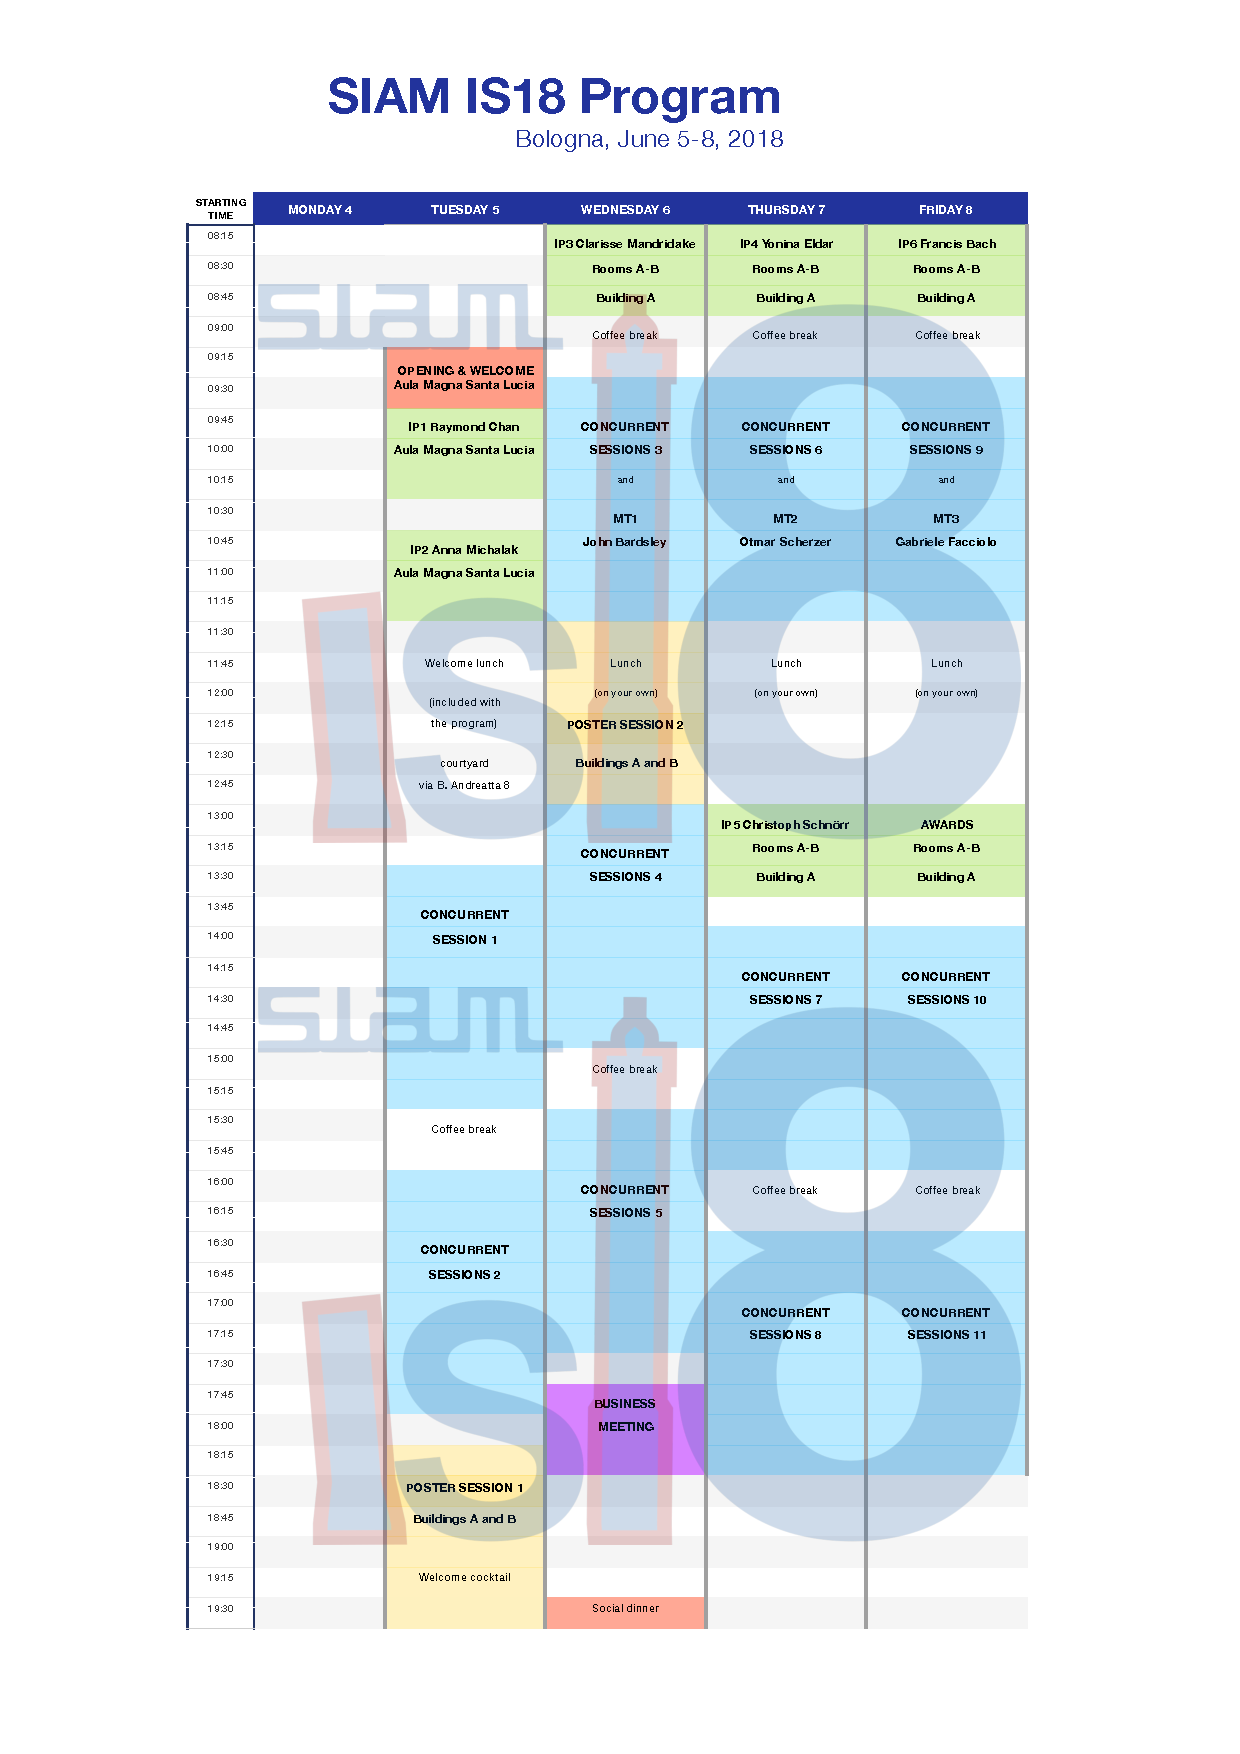
\includegraphics[scale=0.6]{program_table.pdf}

\end{document}
